\section{RNA-Seq}
\subsection{概述}
\begin{frame}
  \frametitle{转录组学 | RNA-Seq | 简介}
  \begin{figure}
    \centering
    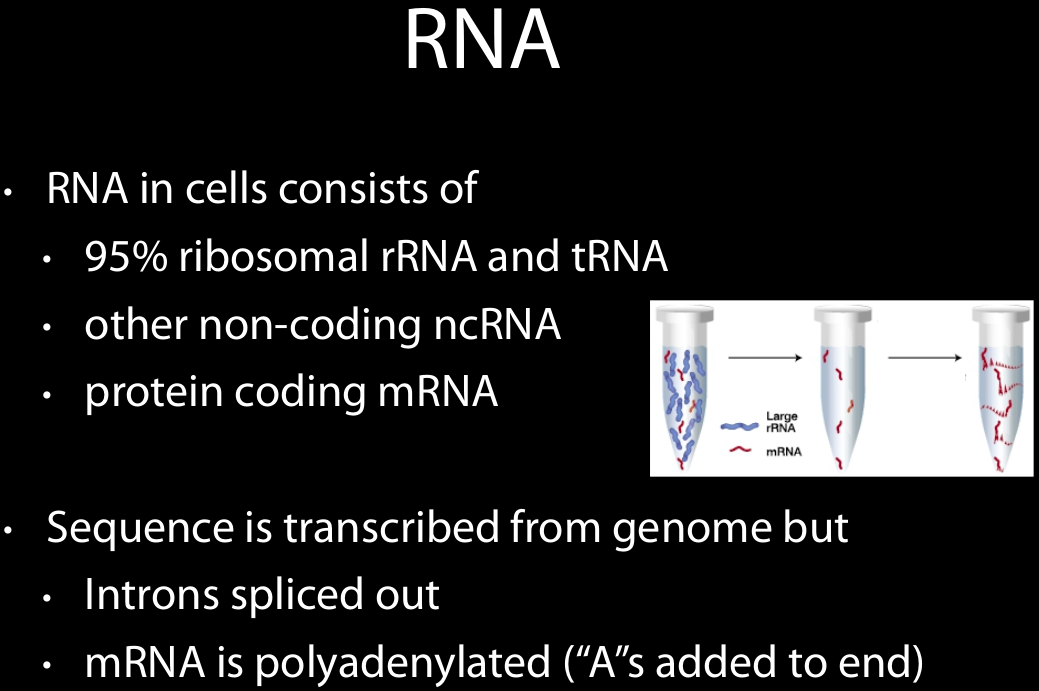
\includegraphics[width=0.9\textwidth]{c3.transcriptome/rna.01.png}
  \end{figure}
\end{frame}

\begin{frame}
  \frametitle{转录组学 | RNA-Seq | 简介}
  \begin{block}{RNA-Seq}
 RNA测序(RNA sequencing,简称RNA-Seq,也被称为全转录物组鸟枪法测序,Whole Transcriptome Shotgun Sequencing,简称WTSS)是基于第二代测序技术的转录组学研究方法。RNA测序是使用第二代测序的能力,在给定时刻从一个基因组中,揭示RNA的存在和数量的一个快照的技术。\\
 \vspace{1em}
RNA-seq (RNA sequencing), also called whole transcriptome shotgun sequencing (WTSS), uses next-generation sequencing (NGS) to reveal the presence and quantity of RNA in a biological sample at a given moment in time.
  \end{block}
\end{frame}

\begin{frame}
  \frametitle{转录组学 | RNA-Seq | 简介}
  \begin{block}{RNA-Seq}
首先提取生物样品的全部转录的RNA,然后反转录为cDNA后进行二代高通量测序,在此基础上进行片段的重叠组装,从而可得到一个个的转录本。\\
\vspace{0.5em}
进而可以形成对该生物样品当前发育状态的基因表达状况的全局了解。\\
\vspace{0.5em}
进一步说,若和下一阶段的生物样品的RNA-Seq转录组进行比较,则可以得到全部的(在转录层面)基因表达的上调及下调——这就形成了表达谱,针对关键基因则可以形成你想要的通路(pathway)的构建。
  \end{block}
\end{frame}

\begin{frame}
  \frametitle{转录组学 | RNA-Seq | 简介}
  \begin{block}{RNA-Seq}
相较于一个静态的染色体而言,细胞内的转录物组是一个处于不断变化的动态过程。随着现在的下一代基因测序(NGS)技术的发展,使得可测得的DNA碱基覆盖面增加且样本输出的吞吐量增大。\\
\vspace{0.5em}
有助于对细胞内RNA转录物进行测序,提供包括选择性剪接转录本、转录后修饰、基因融合、突变/SNPs以及基因表达量改变等细节。\\
\vspace{0.5em}
RNA测序不仅能检测mRNA的转录,还能观测到包括总RNA和小RNA(miRNA、tRNA和核糖体RNA)在内不同RNA群体的表达谱。RNA测序还能用来确定外显子/内含子的边界,修正之前注释的5'和3'端基因边界。未来的RNA测序研究还包括观察感染时细胞传导路径的变化和癌症中不同基因表达程度。
  \end{block}
\end{frame}

\begin{frame}
  \frametitle{转录组学 | RNA-Seq | 简介}
  \begin{block}{技术}
下一代基因测序之前,对转录物组学和基因表达的研究主要基于基因表达芯片(微阵列),后者包含数以千计用于探测靶向序列的DNA探针,可以得到所有表达出转录物的表达谱。基因表达芯片之后,基因表达的系列分析(SAGE)是主要的基因分析技术。\\
\vspace{1em}
Prior to RNA-Seq, gene expression studies were done with hybridization-based microarrays. Issues with microarrays include cross-hybridization artifacts, poor quantification of lowly and highly expressed genes, and needing to know the sequence \textit{a priori}. Because of these technical issues, transcriptomics transitioned to sequencing-based methods. These progressed from Sanger sequencing of Expressed Sequence Tag libraries, to chemical tag-based methods (e.g., serial analysis of gene expression), and finally to the current technology, NGS of cDNA (notably RNA-Seq).
  \end{block}
\end{frame}

\subsection{技术简介}
\begin{frame}
  \frametitle{转录组学 | RNA-Seq | Method | RNA Poly(A) library}
  \begin{block}{poly(A)-poly(T)}
    Frequently, in mRNA analysis the 3' polyadenylated (poly(A)) tail is targeted in order to ensure that coding RNA is separated from noncoding RNA. This can be accomplished simply with poly (T) oligos covalently attached to a given substrate. Presently many studies utilize magnetic beads for this step.
  \end{block}
  \pause
  \begin{block}{poly(T) \& rRNA}
    Studies including portions of the transcriptome outside poly(A) RNAs have shown that when using poly(T) magnetic beads, the flow-through RNA (non-poly(A) RNA) can yield important noncoding RNA gene discovery which would have otherwise gone unnoticed.\\
    \vspace{0.2em}
    Also, since ribosomal RNA represents over 90\% of the RNA within a given cell, studies have shown that its removal via probe hybridization increases the capacity to retrieve data from the remaining portion of the transcriptome.
  \end{block}
\end{frame}

\begin{frame}
  \frametitle{转录组学 | RNA-Seq | Method | RNA Poly(A) library}
  \begin{block}{reverse transcription}
 Due to the 5' bias of randomly primed-reverse transcription as well as secondary structures influencing primer binding sites, hydrolysis of RNA into 200-300 nucleotides prior to reverse transcription reduces both problems simultaneously. However, there are trade-offs with this method where although the overall body of the transcripts are efficiently converted to DNA, the 5' and 3' ends are less so. Depending on the aim of the study, researchers may choose to apply or ignore this step.\\
 \vspace{1em}
    Once the cDNA is synthesized it can be further fragmented to reach the desired fragment length of the sequencing system.
  \end{block}
\end{frame}

\begin{frame}
  \frametitle{转录组学 | RNA-Seq | Method | RNA Poly(A) library}
  \begin{figure}
    \centering
    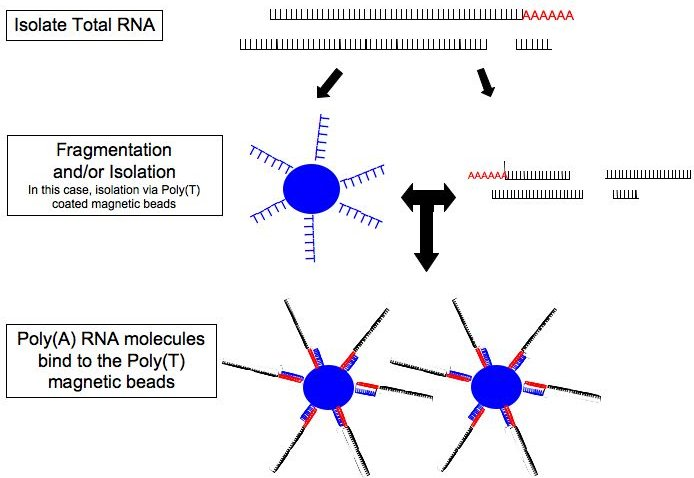
\includegraphics[width=0.48\textwidth]{c3.transcriptome/rs.method.01.jpg}
    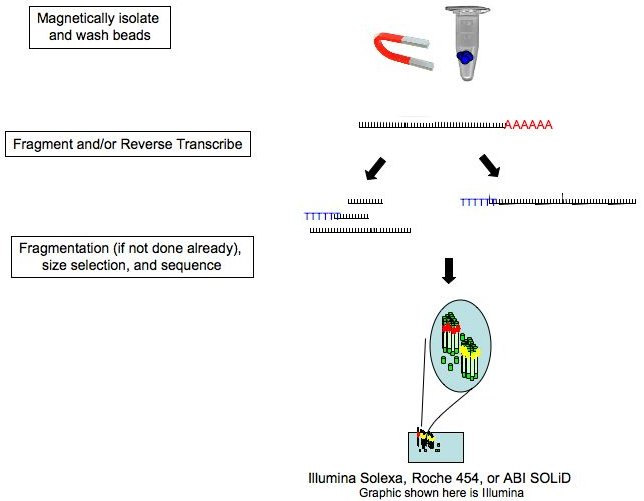
\includegraphics[width=0.46\textwidth]{c3.transcriptome/rs.method.02.jpg}
  \end{figure}
\end{frame}

\begin{frame}
  \frametitle{转录组学 | RNA-Seq | Method | Small RNA/non-coding RNA sequencing}
  \begin{block}{size selection}
 When sequencing RNA other than mRNA, the library preparation is modified. The cellular RNA is selected based on the desired size range. For small RNA targets, such as miRNA, the RNA is isolated through size selection. This can be performed with a size exclusion gel, through size selection magnetic beads, or with a commercially developed kit.\\
 \vspace{1em}
 Once isolated, linkers are added to the 3' and 5' end then purified.\\
 \vspace{1em}
 The final step is cDNA generation through reverse transcription. 
  \end{block}
\end{frame}

\begin{frame}
  \frametitle{转录组学 | RNA-Seq | Method | Direct RNA sequencing}
  \begin{block}{DRSTM}
  As converting RNA into cDNA using reverse transcriptase has been shown to introduce biases and artifacts that may interfere with both the proper characterization and quantification of transcripts, single molecule Direct RNA Sequencing (DRSTM) technology was under development by Helicos (now bankrupt). DRSTM sequences RNA molecules directly in a massively-parallel manner without RNA conversion to cDNA or other biasing sample manipulations such as ligation and amplification.
  \end{block}
\end{frame}

\begin{frame}
  \frametitle{转录组学 | RNA-Seq | Method | Transcriptome assembly}
  \begin{figure}
    \centering
    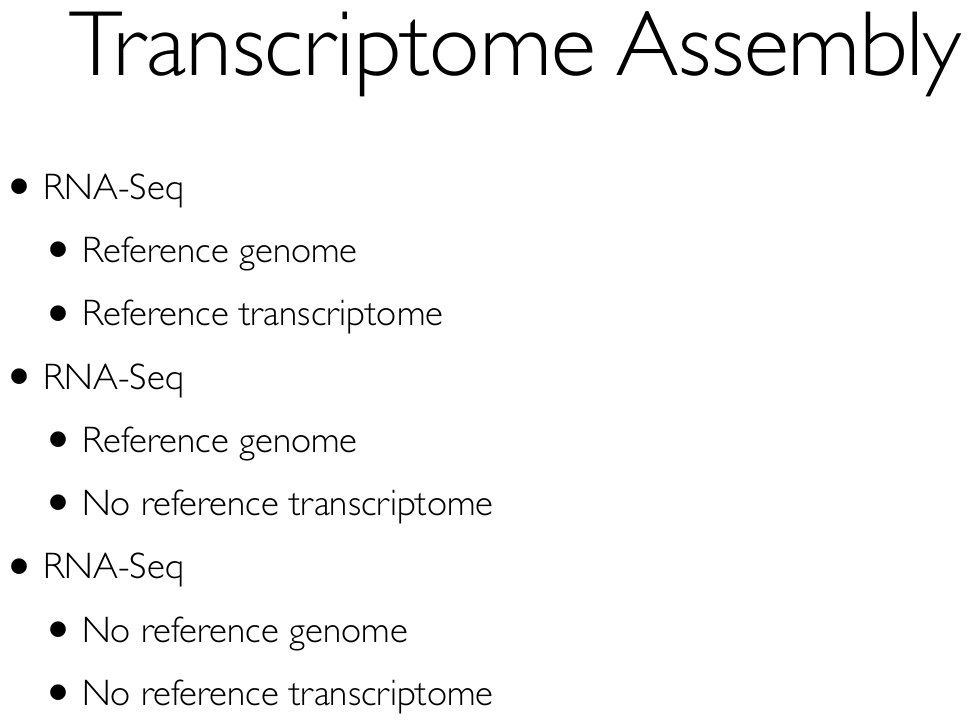
\includegraphics[width=0.8\textwidth]{c3.transcriptome/rs.method.00.png}
  \end{figure}
\end{frame}

\begin{frame}
  \frametitle{转录组学 | RNA-Seq | Method | Transcriptome assembly}
  \begin{block}{2 methods}
    Two different assembly methods are used for producing a transcriptome from raw sequence reads: genome-guided and \textit{de-novo}. 
  \end{block}
  \begin{figure}
    \centering
    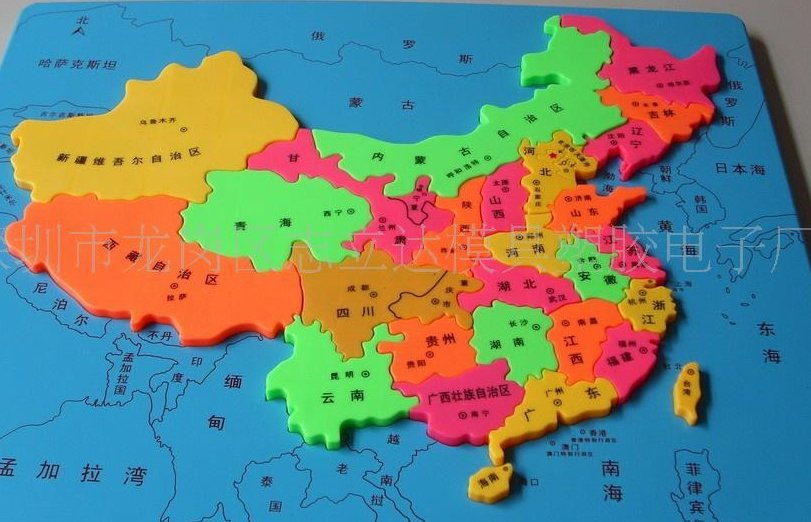
\includegraphics[width=0.42\textwidth]{c3.transcriptome/rs.method.denovo.01.jpg} \quad
    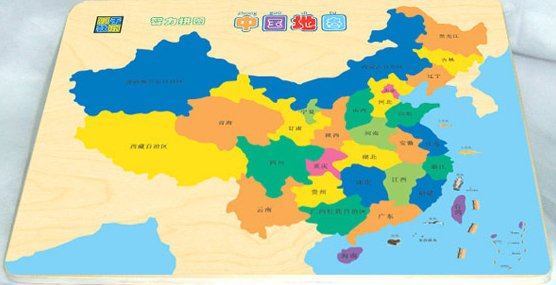
\includegraphics[width=0.53\textwidth]{c3.transcriptome/rs.method.guide.01.jpg}
  \end{figure}
\end{frame}

\begin{frame}
  \frametitle{转录组学 | RNA-Seq | Method | Transcriptome assembly}
  \begin{block}{genome-guided}
    An ``easier" and relatively computationally cheaper approach is that of aligning the millions of reads to a ``reference genome". There are many tools available for aligning genomic reads to a reference genome, however, special attention is needed when aligning a transcriptome to a genome, mainly when dealing with genes having intronic regions. Several software packages exist for short read alignment, and recently specialized algorithms for transcriptome alignment have been developed, e.g. Bowtie for RNA-seq short read alignment, TopHat for aligning reads to a reference genome to discover splice sites, Cufflinks to assemble the transcripts and compare/merge them with others, or FANSe. These tools can also be combined to form a comprehensive system.
  \end{block}
\end{frame}

\begin{frame}
  \frametitle{转录组学 | RNA-Seq | Method | Transcriptome assembly}
  \begin{block}{\textit{de novo}}
    This approach does not rely on the presence of a reference genome in order to reconstruct the nucleotide sequence. Due to the small size of the short reads, \textit{de novo} assembly may be difficult, though some software does exist (Velvet (algorithm), Oases, and Trinity to mention a few), as there cannot be large overlaps between each read needed to easily reconstruct the original sequences. The deep coverage also makes the computing power to track all the possible alignments prohibitive. This deficit can be improved using longer sequences obtained from the same sample using other techniques such as Sanger sequencing, and using larger reads as a ``skeleton" or a ``template" to help assemble reads in difficult regions (e.g. regions with repetitive sequences).
  \end{block}
\end{frame}

\begin{frame}
  \frametitle{转录组学 | RNA-Seq | Method | Transcriptome assembly}
  \begin{block}{Notes}
    \begin{itemize}
      \item assembly quality can vary a lot depending on which metric is used
      \item assemblies that scored well in one species did not really perform well in the other species
      \item the ``most reliable" assembly could be then obtained by combining different approaches
    \end{itemize}
  \end{block}
\end{frame}

\begin{frame}
  \frametitle{转录组学 | RNA-Seq | Method | Transcriptome assembly}
  \begin{block}{junction}
 The created library and the short reads obtained cannot come from intronic sequences, so library reads spanning the junction of two or more exons will not align to the genome.\\
 \vspace{1em}
 A possible method to work around this is to try to align the unaligned short reads using a proxy genome generated with known exonic sequences. This need not cover whole exons, only enough so that the short reads can match on both sides of the exon-exon junction with minimum overlap.
  \end{block}
\end{frame}

\begin{frame}
  \frametitle{转录组学 | RNA-Seq | Method | Transcriptome assembly}
  \begin{figure}
    \centering
    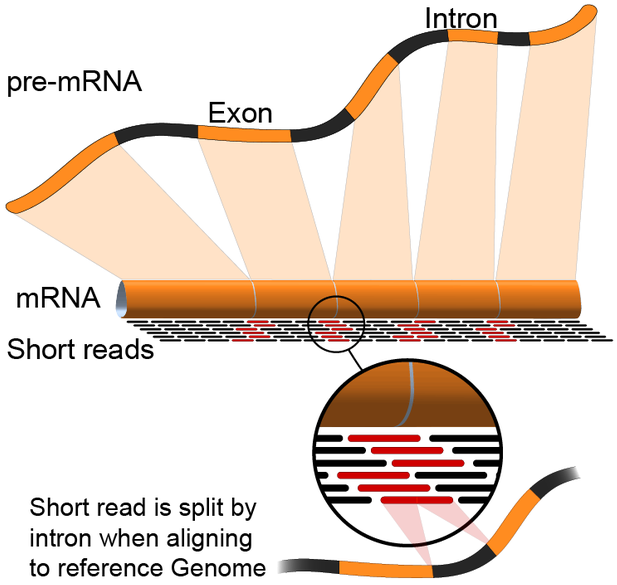
\includegraphics[width=0.55\textwidth]{c3.transcriptome/rs.method.guide.intron.01.png}
  \end{figure}
\end{frame}

\begin{frame}
  \frametitle{转录组学 | RNA-Seq | Method | Transcriptome assembly}
  \begin{figure}
    \centering
    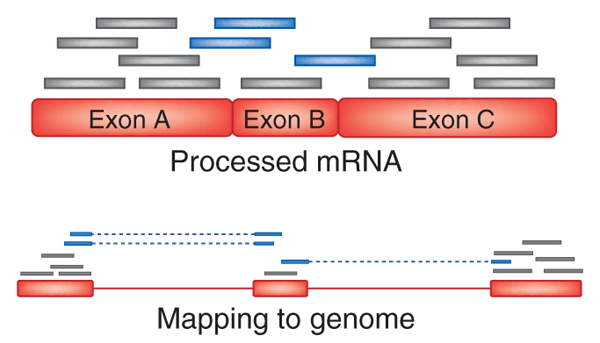
\includegraphics[width=0.9\textwidth]{c3.transcriptome/rs.method.guide.intron.02.png}
  \end{figure}
\end{frame}

\begin{frame}
  \frametitle{转录组学 | RNA-Seq | Method | Experimental considerations}
  {\footnotesize
  \begin{block}{pros \& cons}
    \begin{itemize}
      \item Tissue specificity: Gene expression is not uniform throughout an organism's cells, it is strongly dependent on the tissue type being measured. RNA-Seq can provide a complete snapshot of all the transcripts being available at that precise moment in the cell.
      \item Time dependent: During a cell's lifetime and context, its gene expression levels change. Any single sequencing experiment will offer information regarding one point in time.
      \item Coverage: coverage/depth can affect the mutations seen.
      \item Subjectivity of the analysis: Numerous attempts have been taken to uniformly analyze the data. However, the results can vary due to the multitude of algorithms and pipelines available.
      \item Data management: The main issue with NGS data is the volume of data produced.
      \item Downstream interpretation of the data: Different layers of interpretations have to be considered when analyzing RNA-Seq data.
    \end{itemize}
  \end{block}
  }
\end{frame}

\begin{frame}
  \frametitle{转录组学 | RNA-Seq | Application}
  \begin{figure}
    \centering
    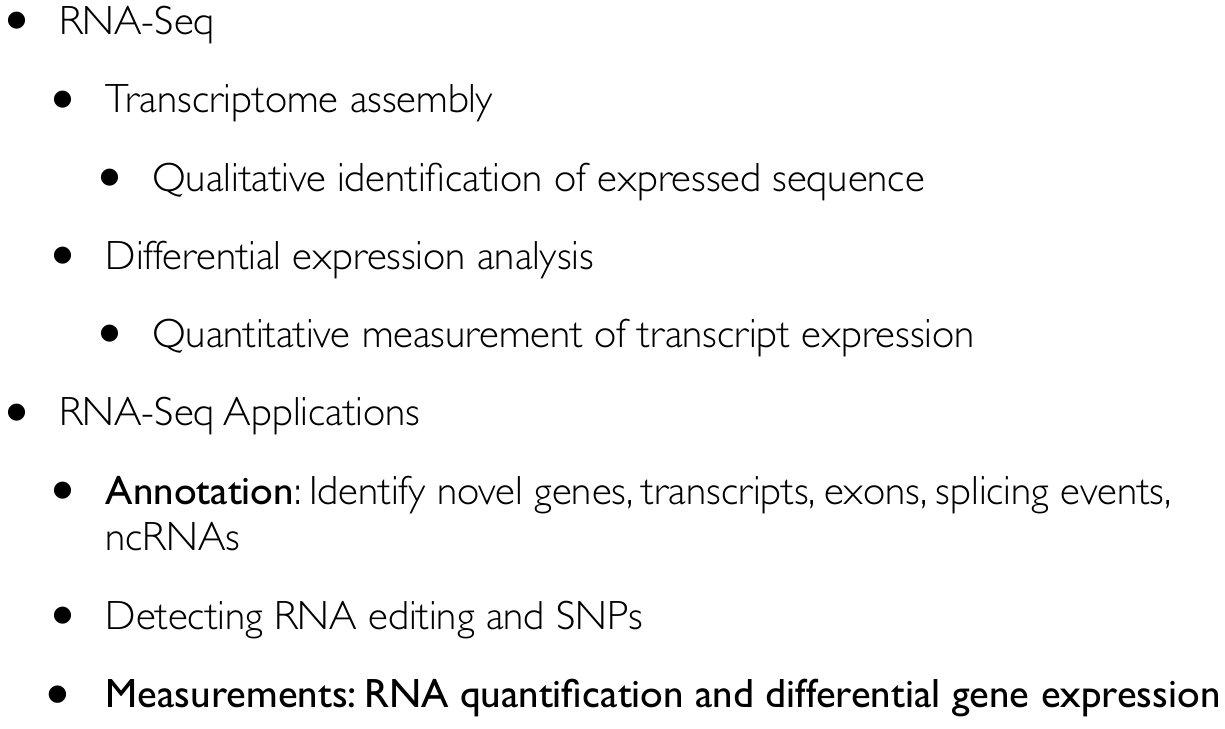
\includegraphics[width=0.9\textwidth]{c3.transcriptome/rs.application.00.png}
  \end{figure}
\end{frame}

\begin{frame}
  \frametitle{转录组学 | RNA-Seq | Application}
  \begin{figure}
    \centering
    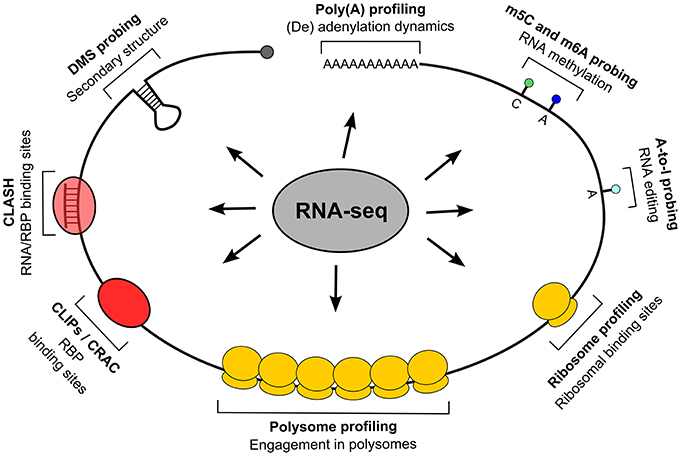
\includegraphics[width=0.9\textwidth]{c3.transcriptome/rs.application.01.jpg}
  \end{figure}
\end{frame}

\begin{frame}
  \frametitle{转录组学 | RNA-Seq | Application}
  \begin{figure}
    \centering
    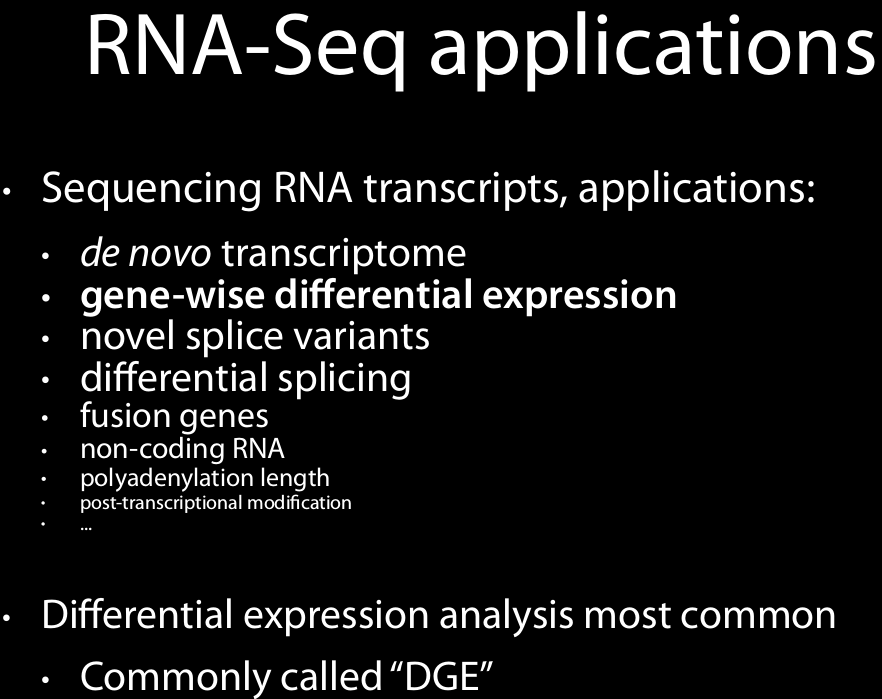
\includegraphics[width=0.8\textwidth]{c3.transcriptome/rs.application.02.png}
  \end{figure}
\end{frame}

\begin{frame}
  \frametitle{转录组学 | RNA-Seq | Application}
  \begin{figure}
    \centering
    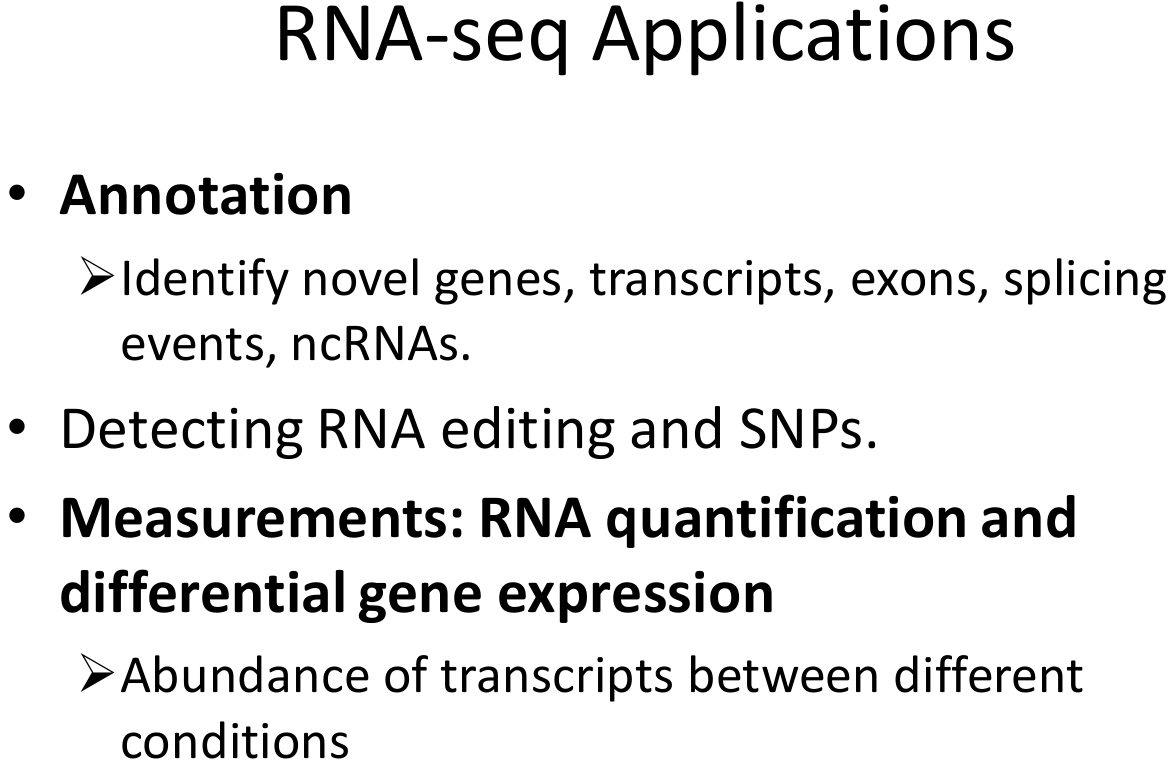
\includegraphics[width=0.9\textwidth]{c3.transcriptome/rs.application.03.png}
  \end{figure}
\end{frame}

\begin{frame}
  \frametitle{转录组学 | RNA-Seq | Application}
  \begin{figure}
    \centering
    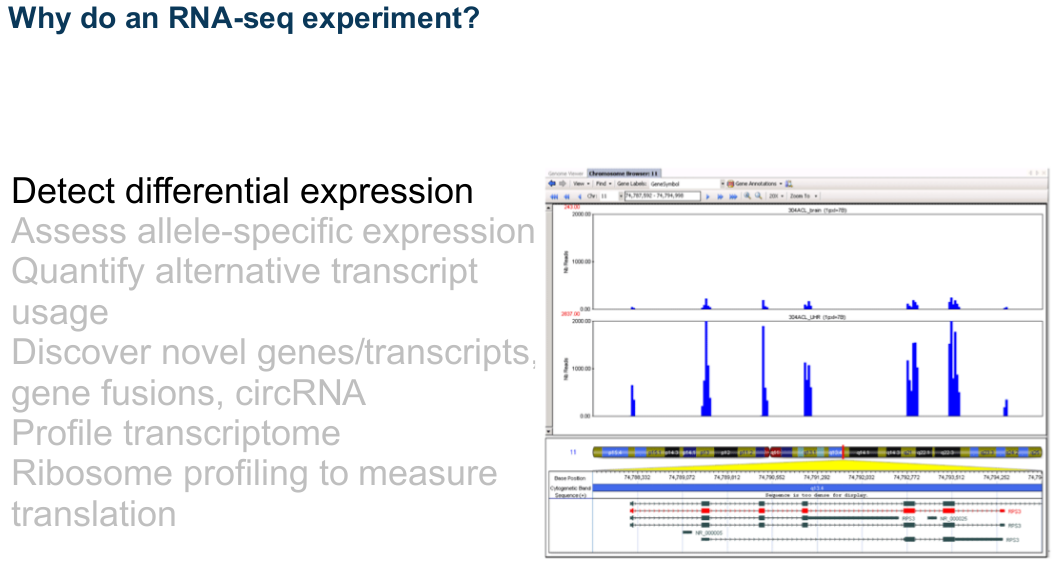
\includegraphics[width=0.9\textwidth]{c3.transcriptome/rs.application.10.png}
  \end{figure}
\end{frame}

\begin{frame}
  \frametitle{转录组学 | RNA-Seq | Application}
  \begin{figure}
    \centering
    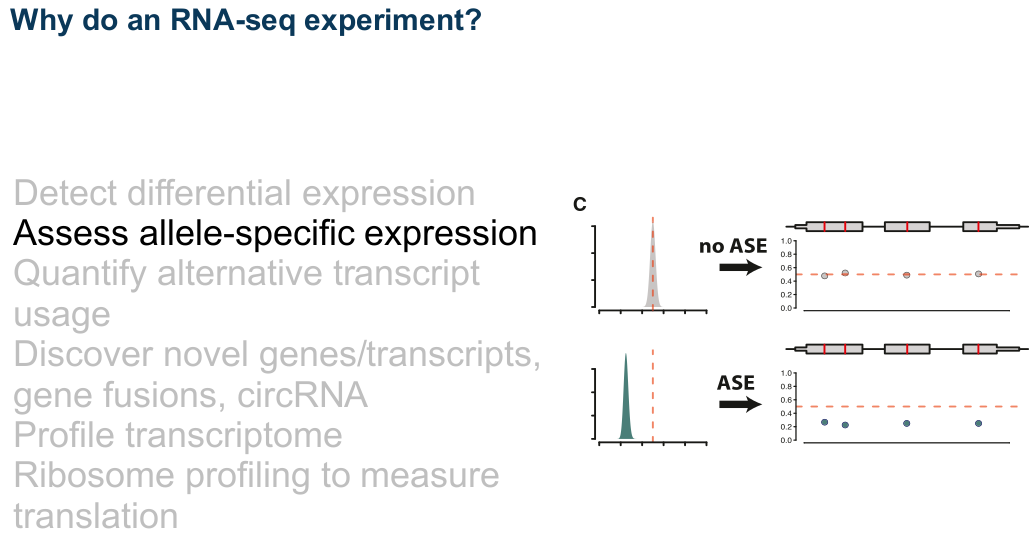
\includegraphics[width=0.9\textwidth]{c3.transcriptome/rs.application.11.png}
  \end{figure}
\end{frame}

\begin{frame}
  \frametitle{转录组学 | RNA-Seq | Application}
  \begin{figure}
    \centering
    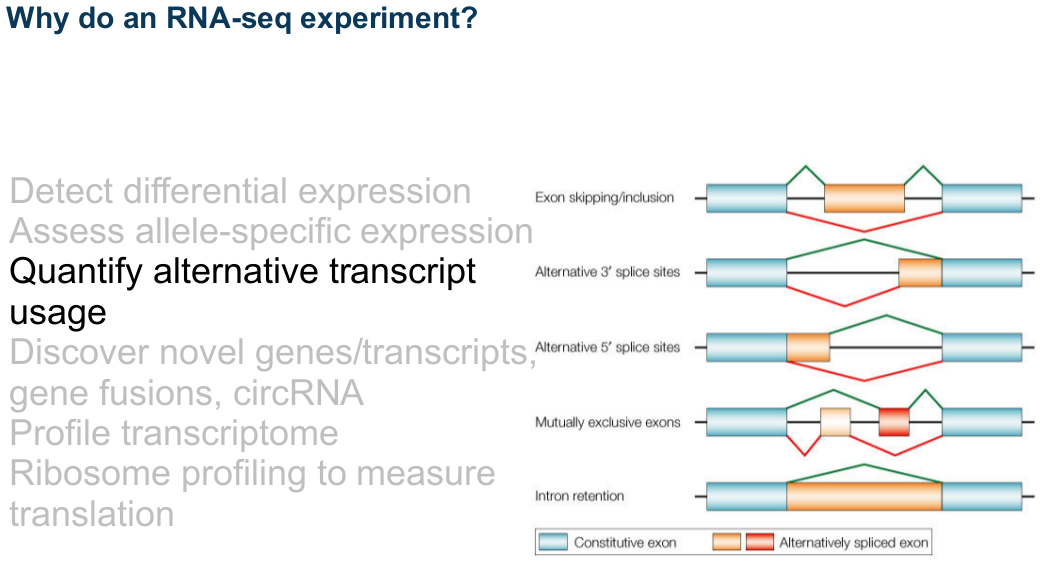
\includegraphics[width=0.9\textwidth]{c3.transcriptome/rs.application.12.png}
  \end{figure}
\end{frame}

\begin{frame}
  \frametitle{转录组学 | RNA-Seq | Application}
  \begin{figure}
    \centering
    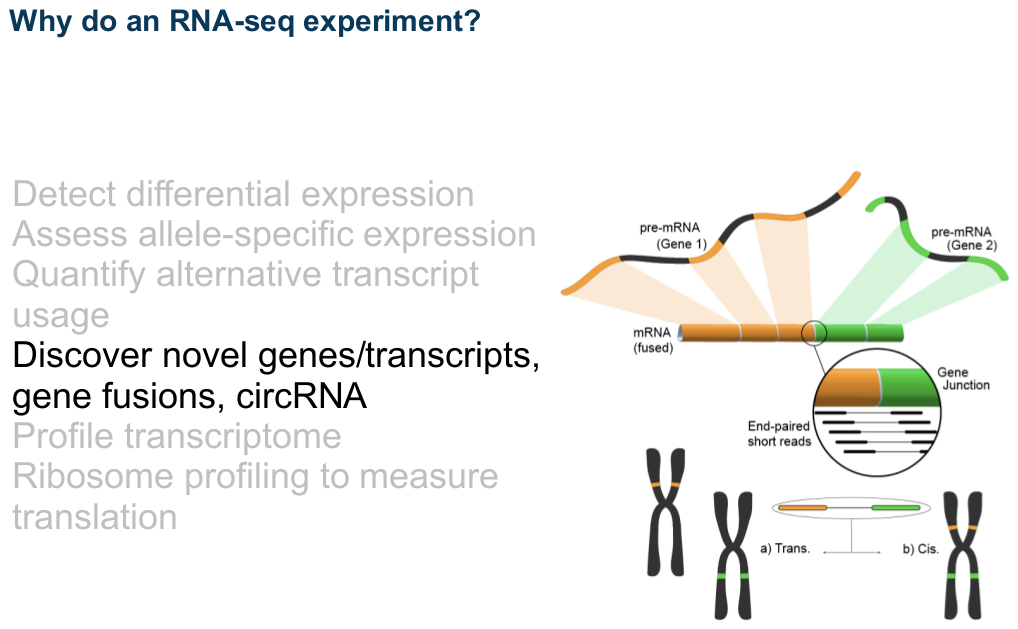
\includegraphics[width=0.9\textwidth]{c3.transcriptome/rs.application.13.png}
  \end{figure}
\end{frame}

\begin{frame}
  \frametitle{转录组学 | RNA-Seq | Application}
  \begin{figure}
    \centering
    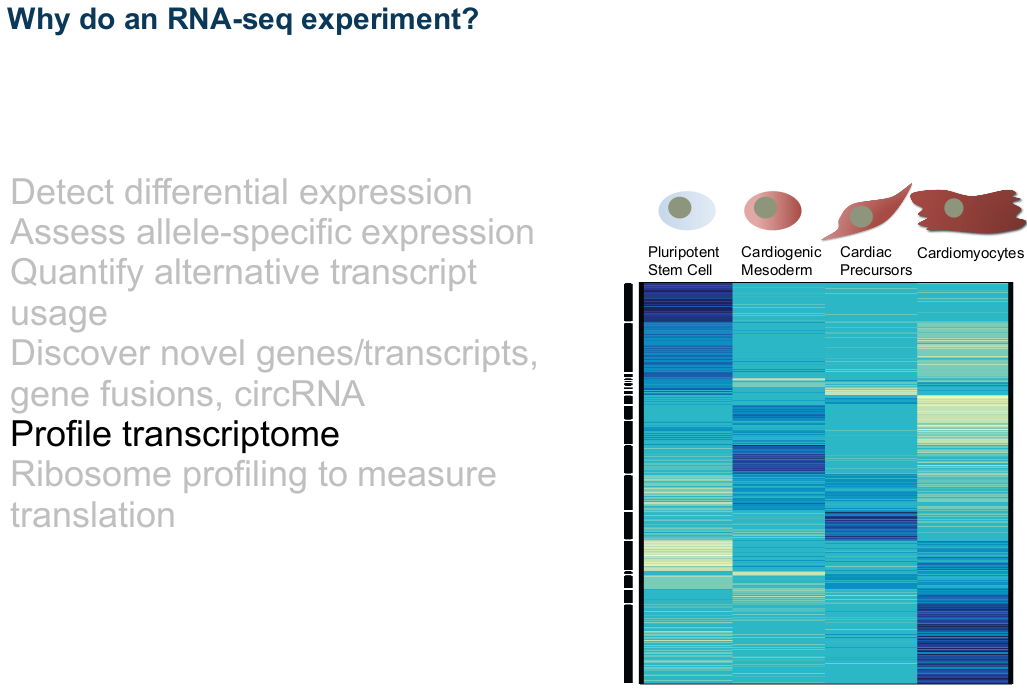
\includegraphics[width=0.9\textwidth]{c3.transcriptome/rs.application.14.png}
  \end{figure}
\end{frame}

\begin{frame}
  \frametitle{转录组学 | RNA-Seq | Application}
  \begin{figure}
    \centering
    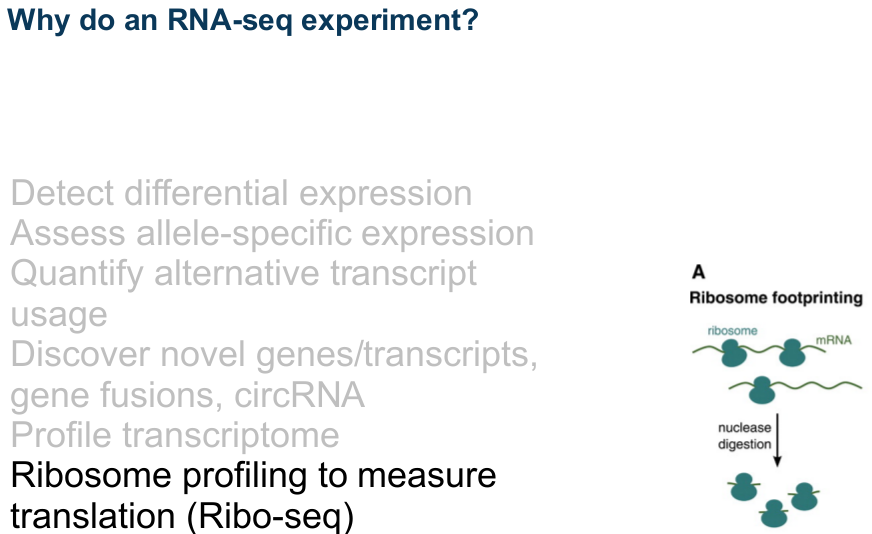
\includegraphics[width=0.9\textwidth]{c3.transcriptome/rs.application.15.png}
  \end{figure}
\end{frame}

\begin{frame}
  \frametitle{转录组学 | RNA-Seq | Experiment}
  \begin{figure}
    \centering
    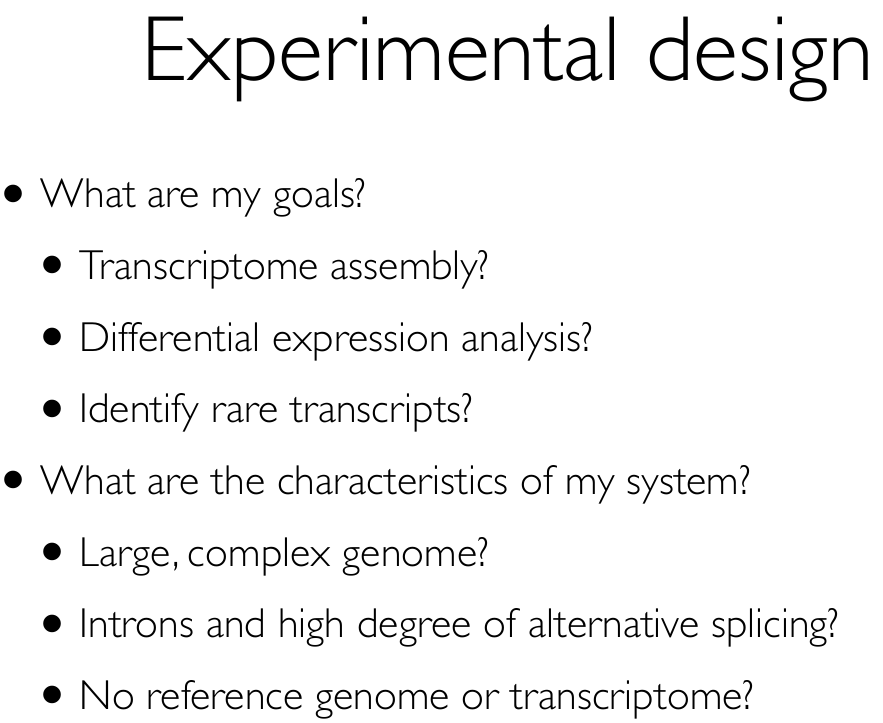
\includegraphics[width=0.8\textwidth]{c3.transcriptome/rs.experiment.01.png}
  \end{figure}
\end{frame}

\begin{frame}
  \frametitle{转录组学 | RNA-Seq | Experiment}
  \begin{figure}
    \centering
    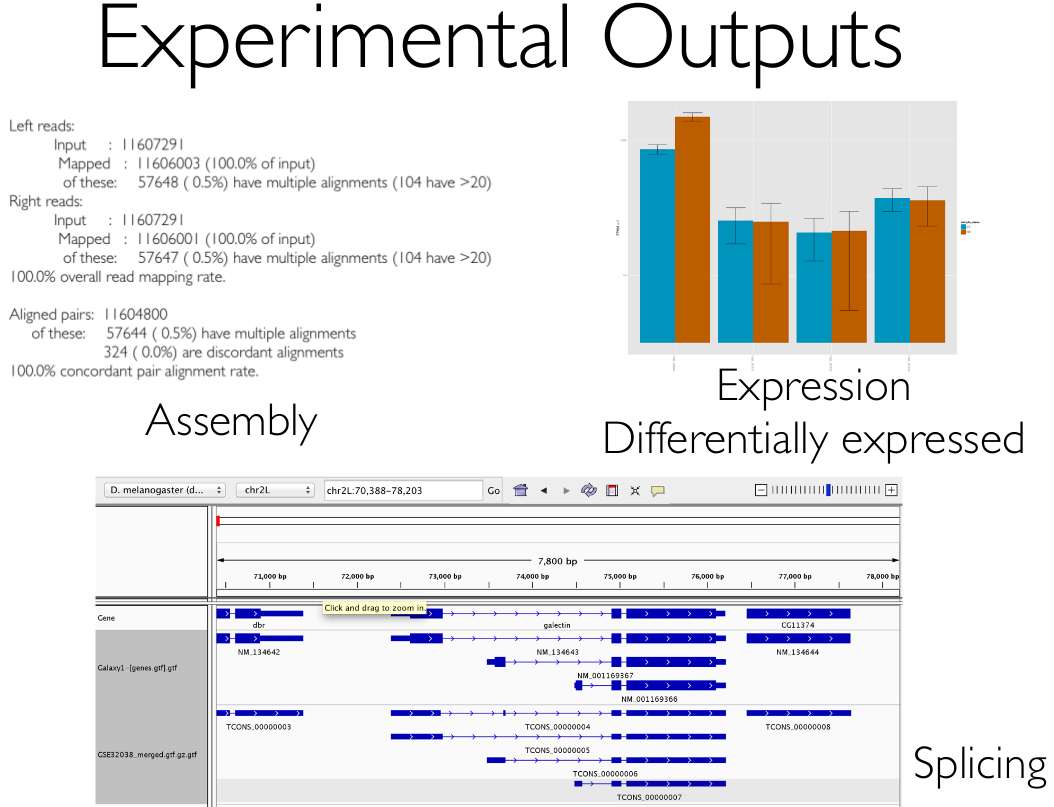
\includegraphics[width=0.8\textwidth]{c3.transcriptome/rs.experiment.02.png}
  \end{figure}
\end{frame}

\begin{frame}
  \frametitle{转录组学 | RNA-Seq | Analysis}
  \begin{figure}
    \centering
    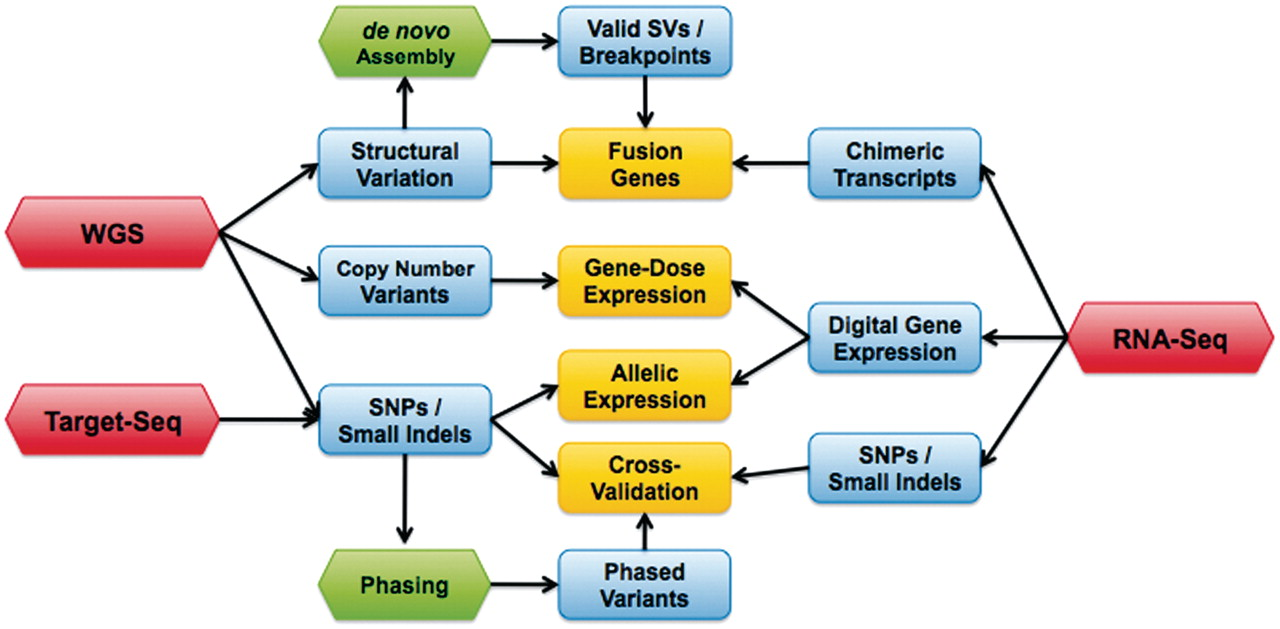
\includegraphics[width=\textwidth]{c3.transcriptome/rs.analysis.02.jpg}
  \end{figure}
\end{frame}

\begin{frame}
  \frametitle{转录组学 | RNA-Seq | Analysis | Workflow}
  \begin{figure}
    \centering
    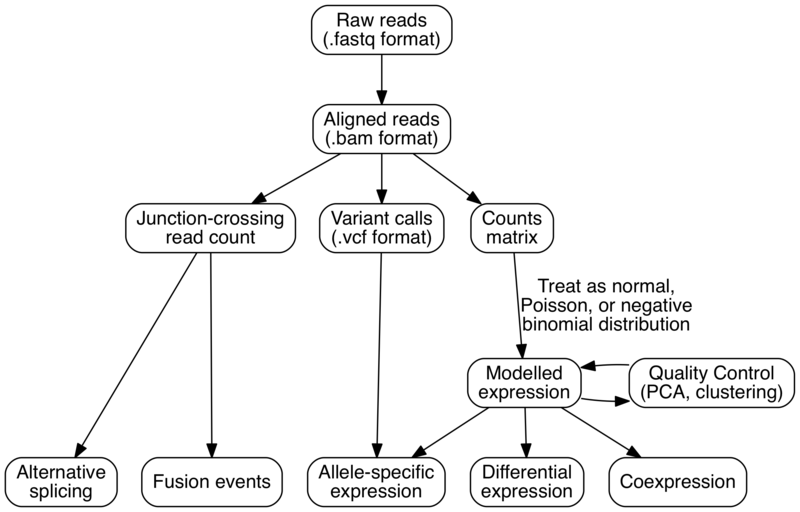
\includegraphics[width=0.9\textwidth]{c3.transcriptome/rs.analysis.workflow.01.png}
  \end{figure}
\end{frame}

\begin{frame}
  \frametitle{转录组学 | RNA-Seq | Analysis | Gene expression}
  \begin{block}{Gene expression}
    \begin{itemize}
      \item Which genes are expressed in what tissues, and at what levels.
      \item Measuring mRNA concentration levels is a useful tool in determining how the transcriptional machinery of the cell is affected in the presence of external signals (e.g. drug treatment), or how cells differ between a healthy state and a diseased state.
      \item Expression levels are expressed as Fragments Per Kilobase of transcript per Million mapped reads (FPKM).
      \item An R-based statistical package known as CummeRbund can be used to generate expression comparison charts for visual analysis.
    \end{itemize}
  \end{block}
\end{frame}

\begin{frame}
  \frametitle{转录组学 | RNA-Seq | Analysis | Gene expression}
  \begin{figure}
    \centering
    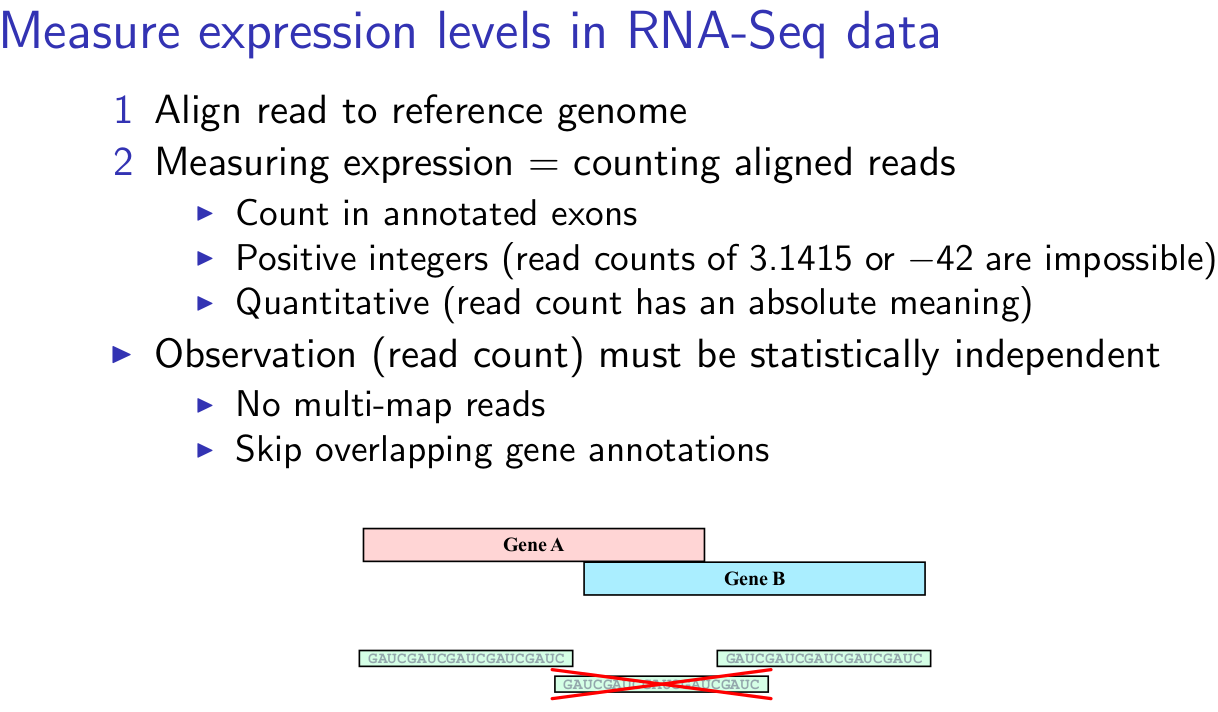
\includegraphics[width=\textwidth]{c3.transcriptome/rs.exp.01.png}
  \end{figure}
\end{frame}

\begin{frame}
  \frametitle{转录组学 | RNA-Seq | Analysis | Differential expression}
  \begin{block}{Differential expression}
 RNA-Seq is generally used to compare gene expression between conditions, such as a drug treatment vs non-treated, and find out which genes are up- or down regulated in each condition.\\
 \vspace{0.5em}
 Differently expressed genes can be identified by using tools that count the sequencing reads per gene and compare them between samples. The most commonly used tools for this type of analysis are DESeq and edgeR, packages from Bioconductor. Both these tools use a model based on the negative binomial distribution.
  \end{block}
\end{frame}

\begin{frame}
  \frametitle{转录组学 | RNA-Seq | Analysis | Differential expression}
  \begin{figure}
    \centering
    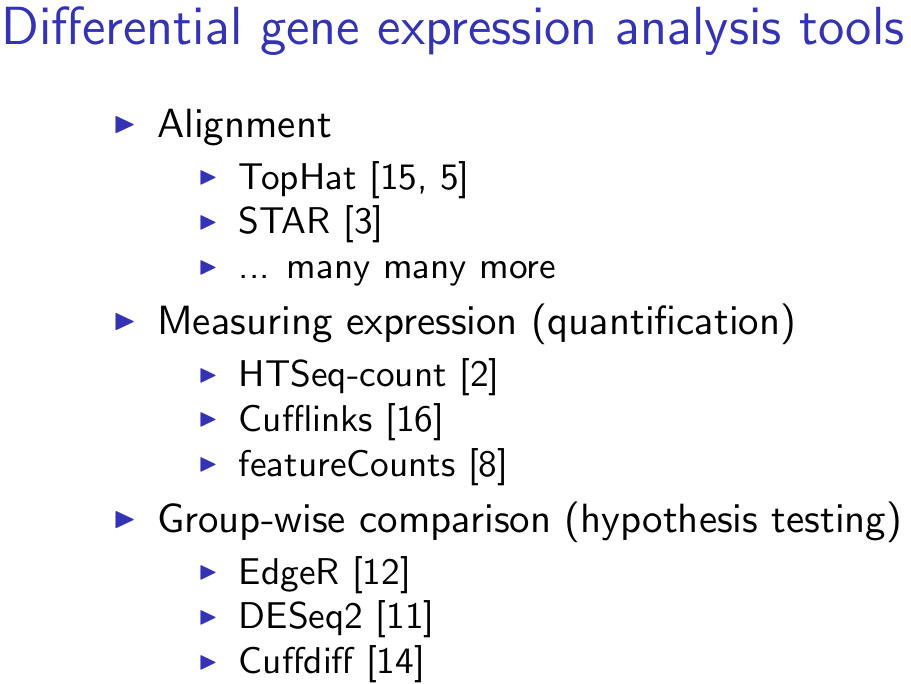
\includegraphics[width=0.85\textwidth]{c3.transcriptome/rs.deg.01.png}
  \end{figure}
\end{frame}

\begin{frame}
  \frametitle{转录组学 | RNA-Seq | Analysis | Differential expression}
  \begin{figure}
    \centering
    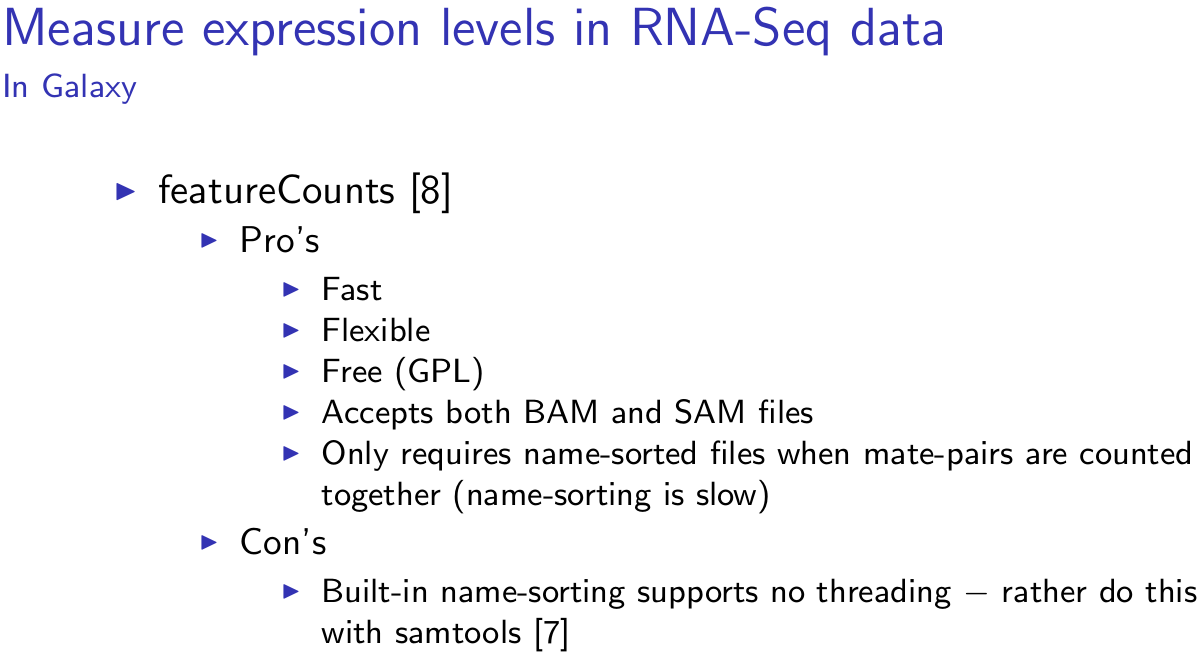
\includegraphics[width=\textwidth]{c3.transcriptome/rs.deg.02.png}
  \end{figure}
\end{frame}

\begin{frame}
  \frametitle{转录组学 | RNA-Seq | Analysis | Differential expression}
  \begin{figure}
    \centering
    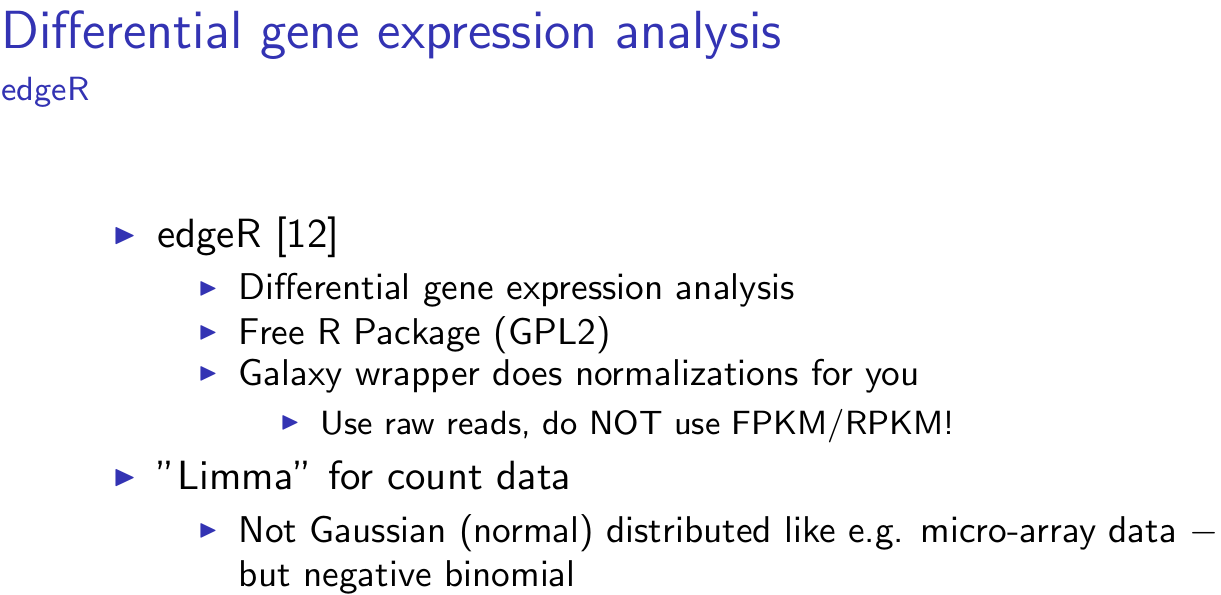
\includegraphics[width=\textwidth]{c3.transcriptome/rs.deg.03.png}
  \end{figure}
\end{frame}

\begin{frame}
  \frametitle{转录组学 | RNA-Seq | Analysis | Absolute quantification of transcripts}
  \begin{block}{Absolute quantification of transcripts}
 It is not possible to do absolute quantification using the common RNA-Seq pipeline, because it only provides RNA levels relative to all transcripts. If the total amount of RNA in the cell changes between conditions, relative normalization will misrepresent the changes for individual transcripts. Absolute quantification of mRNAs is possible by performing RNA-Seq with added spike ins, samples of RNA at known concentrations. After sequencing, the read count of the spike ins sequences is used to determine the direct correspondence between read count and biological fragments.
  \end{block}
\end{frame}

\begin{frame}
  \frametitle{转录组学 | RNA-Seq | Analysis | SNV discovery}
  \begin{block}{SNV discovery}
    RNA-seq is limited to transcribed regions however, since it will only discover sequence variations in exon regions. This misses many subtle but important intron alleles that affect disease such as transcription regulators, leaving analysis to only large effectors. While some correlation exists between exon to intron variation, only whole genome sequencing would be able to capture the source of all relevant SNPs.
  \end{block}
\end{frame}

\begin{frame}
  \frametitle{转录组学 | RNA-Seq | Analysis | SNV discovery}
  \begin{figure}
    \centering
    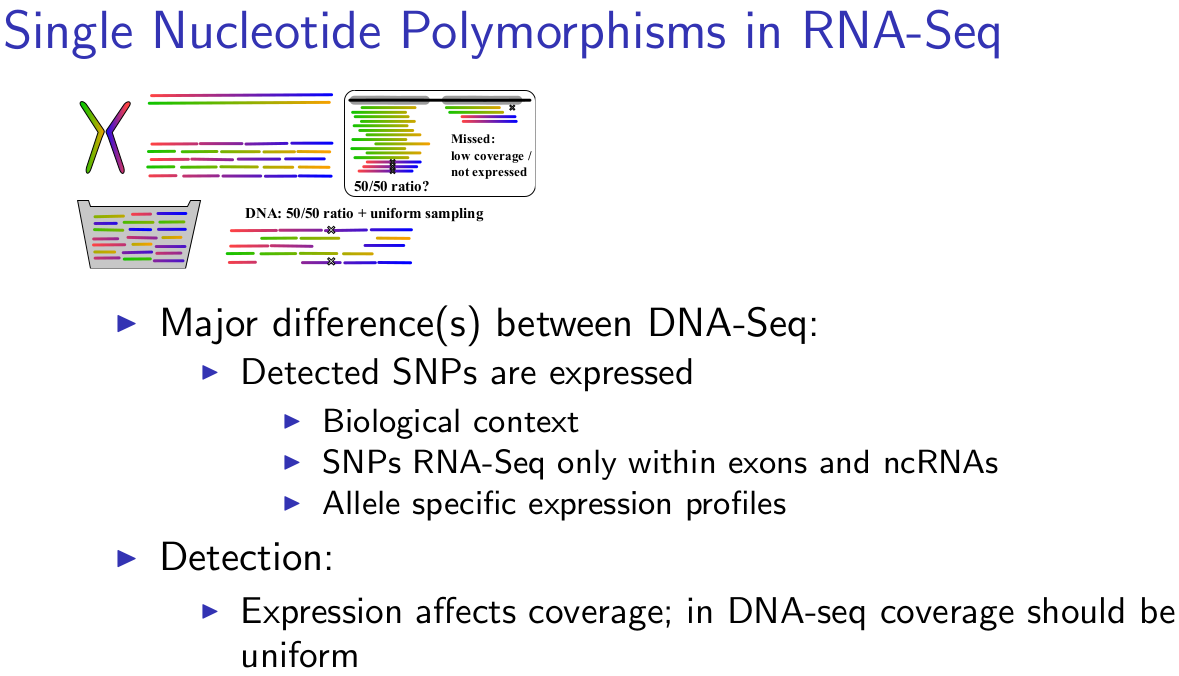
\includegraphics[width=0.9\textwidth]{c3.transcriptome/rs.snv.01.png}
  \end{figure}
\end{frame}

\begin{frame}
  \frametitle{转录组学 | RNA-Seq | Analysis | SNV discovery}
  \begin{figure}
    \centering
    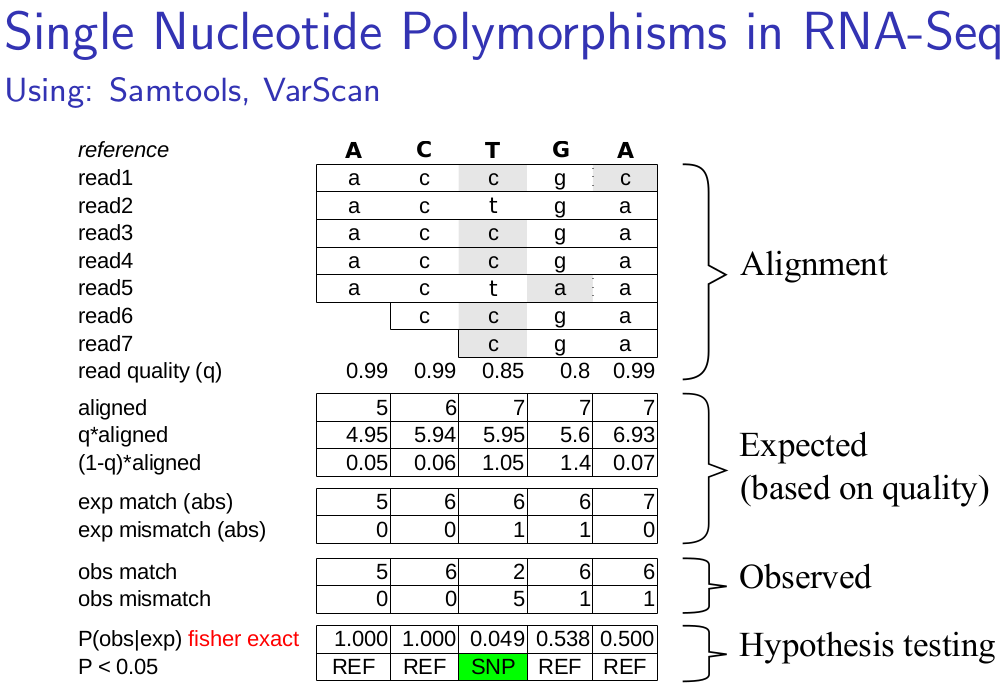
\includegraphics[width=0.9\textwidth]{c3.transcriptome/rs.snv.02.png}
  \end{figure}
\end{frame}

\begin{frame}
  \frametitle{转录组学 | RNA-Seq | Analysis | SNV discovery}
  \begin{figure}
    \centering
    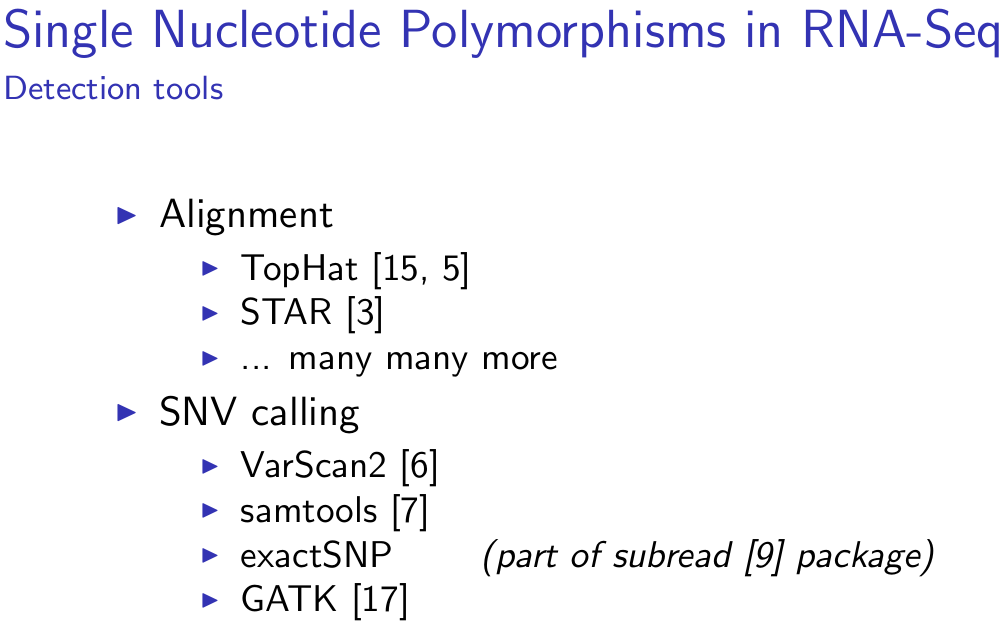
\includegraphics[width=0.9\textwidth]{c3.transcriptome/rs.snv.03.png}
  \end{figure}
\end{frame}

\begin{frame}
  \frametitle{转录组学 | RNA-Seq | Analysis | Post-transcriptional edits}
  \begin{block}{Post-transcriptional edits}
    Having the matching genomic and transcriptomic sequences of an individual can also help in detecting post-transcriptional edits, where, if the individual is homozygous for a gene, but the gene's transcript has a different allele, then a post-transcriptional modification event is determined.\\
    \vspace{1em}
    mRNA centric single nucleotide variants (SNVs) are generally not considered as a representative source of functional variation in cells, mainly due to the fact that these mutations disappear with the mRNA molecule, however the fact that efficient DNA correction mechanisms do not apply to RNA molecules can cause them to appear more often. This has been proposed as the source of certain prion diseases, also known as TSE or transmissible spongiform encephalopathies.
  \end{block}
\end{frame}

\begin{frame}
  \frametitle{转录组学 | RNA-Seq | Analysis | Fusion gene detection}
  {\footnotesize
  \begin{block}{Fusion gene detection}
  Caused by different structural modifications in the genome, fusion genes have gained attention because of their relationship with cancer. The ability of RNA-seq to analyze a sample's whole transcriptome in an unbiased fashion makes it an attractive tool to find these kinds of common events in cancer.\\
  \vspace{0.5em}
  The idea follows from the process of aligning the short transcriptomic reads to a reference genome. Most of the short reads will fall within one complete exon, and a smaller but still large set would be expected to map to known exon-exon junctions. The remaining unmapped short reads would then be further analyzed to determine whether they match an exon-exon junction where the exons come from different genes. This would be evidence of a possible fusion event, however, because of the length of the reads, this could prove to be very noisy. An alternative approach is to use pair-end reads, when a potentially large number of paired reads would map each end to a different exon, giving better coverage of these events. Nonetheless, the end result consists of multiple and potentially novel combinations of genes providing an ideal starting point for further validation.
  \end{block}
  }
\end{frame}

\begin{frame}
  \frametitle{转录组学 | RNA-Seq | Analysis | Fusion gene detection}
  \begin{figure}
    \centering
    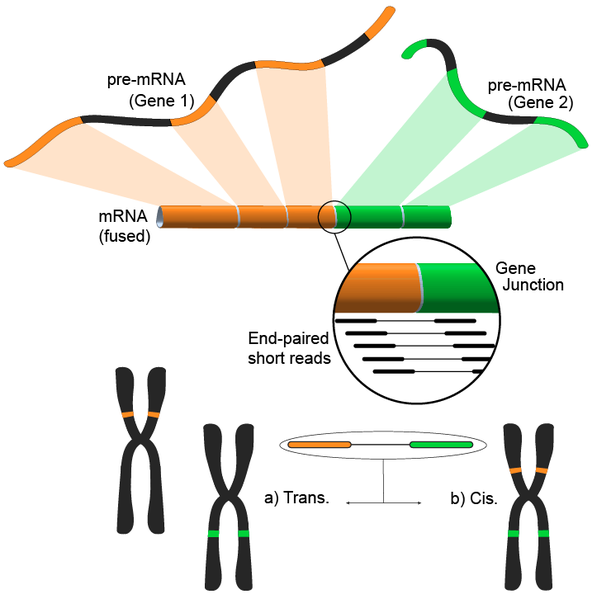
\includegraphics[width=0.6\textwidth]{c3.transcriptome/rs.analysis.fusion.01.png}
  \end{figure}
\end{frame}

\begin{frame}
  \frametitle{转录组学 | RNA-Seq | Analysis | Coexpression networks}
  \begin{block}{Coexpression networks}
    Coexpression networks are data-derived representations of genes behaving in a similar way across tissues and experimental conditions. Their main purpose lies in hypothesis generation and guilt-by-association approaches for inferring functions of previously unknown genes. RNA-Seq data has been recently used to infer genes involved in specific pathways based on Pearson correlation, both in plants and mammals. The main advantage of RNA-Seq data in this kind of analysis over the microarray platforms is the capability to cover the entire transcriptome, therefore allowing the possibility to unravel more complete representations of the gene regulatory networks.\\
 \vspace{0.5em}
 Co-expression modules may corresponds to cell types or pathways. Highly connected intramodular hubs can be interpreted as representatives of their respective module.
  \end{block}
\end{frame}

\begin{frame}
  \frametitle{转录组学 | RNA-Seq | Application}
  \begin{block}{Application to genomic medicine}
  RNA-Seq data could help researchers interpreting the ``personalized transcriptome" so that it will help understanding the transcriptomic changes happening therefore, ideally, identifying gene drivers for a disease. The feasibility of this approach is however dictated by the costs in terms of money and time.\\
  \vspace{1em}
  RNA-Seq applications to the clinic have the potentials to significantly affect patient's life and, on the other hand, requires a team of specialists (bioinformaticians, physicians/clinicians, basic researchers, technicians) to fully interpret the huge amount of data generated by this analysis.
  \end{block}
\end{frame}

\begin{frame}
  \frametitle{转录组学 | RNA-Seq | Application}
  \begin{block}{Application to genomic medicine}
    Compared with microarrays, NGS technology has identified \textcolor{red}{novel and low frequency RNAs} associated with disease processes. This advantage aids in the diagnosis and possible future treatments of diseases, including cancer. Numerous studies have demonstrated NGS's ability to detect aberrant mRNA and small non-coding RNA expression in disease processes above that provided by microarrays. The lower cost and higher throughput offered by NGS confers another advantage to researchers.\\
  \vspace{1em}
  The role of small non-coding RNAs in disease processes has also been explored in recent years.
  \end{block}
\end{frame}

\begin{frame}
  \frametitle{转录组学 | RNA-Seq | Databases}
  \begin{block}{ENCODE \& TCGA}
 A lot of emphasis has been given to RNA-Seq data after the Encyclopedia of the regulatory elements (ENCODE) and The Cancer Genome Atlas (TCGA) projects have used this approach to characterize dozens of cell lines and thousands of primary tumor samples, respectively.\\
 \vspace{1em}
 RNA-Seq data provide a unique snapshot of the transcriptomic status of the disease and look at an unbiased population of transcripts that allows the identification of novel transcripts, fusion transcripts and non-coding RNAs that could be undetected with different technologies.
  \end{block}
\end{frame}

\begin{frame}
  \frametitle{转录组学 | RNA-Seq | Databases}
  \begin{block}{ENCODE}
    ENCODE aimed to identify genome-wide regulatory regions in different cohort of cell lines and transcriptomic data are paramount in order to understand the downstream effect of those epigenetic and genetic regulatory layers.
  \end{block}
  \pause
  \begin{block}{TCGA}
    TCGA aimed to collect and analyze thousands of patient's samples from 30 different tumor types in order to understand the underlying mechanisms of malignant transformation and progression.
  \end{block}
\end{frame}

\begin{frame}
  \frametitle{转录组学 | RNA-Seq | Databases | ENCODE}
  \begin{figure}
    \centering
    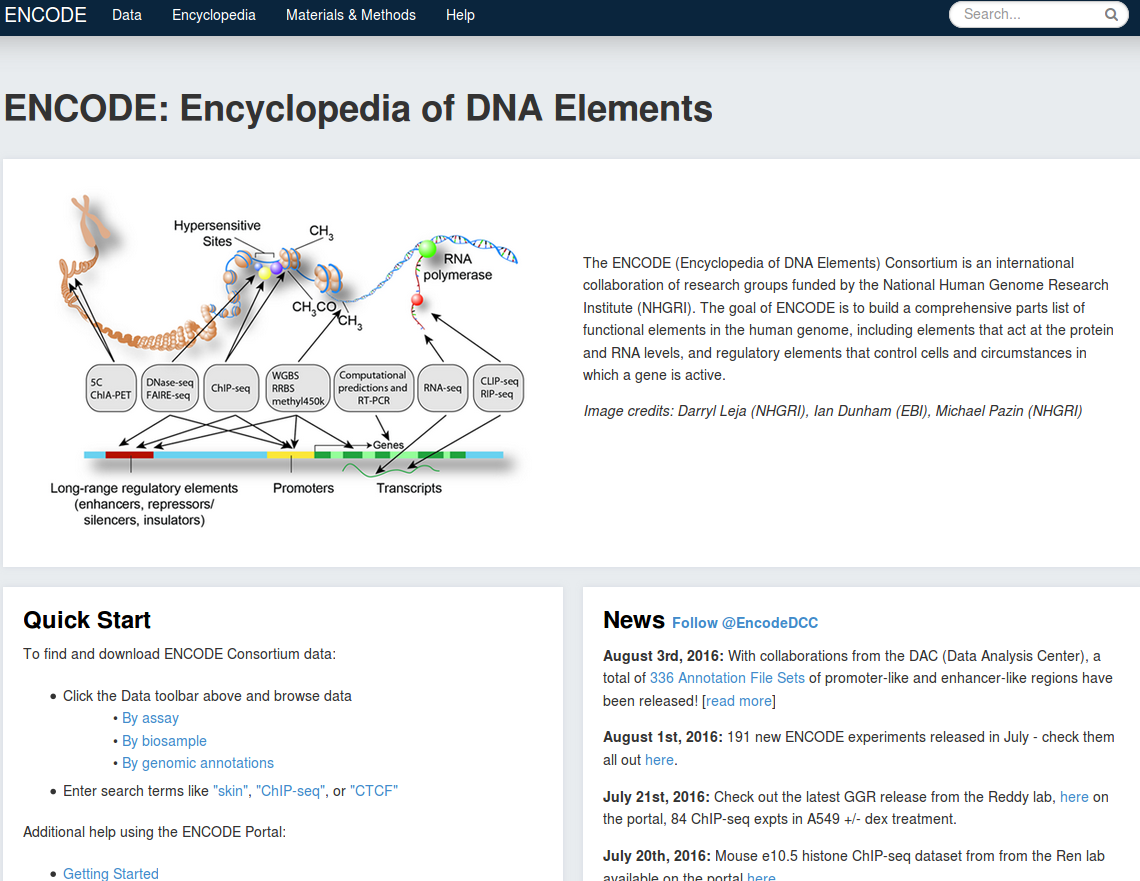
\includegraphics[width=0.8\textwidth]{c3.transcriptome/db.encode.01.png}
  \end{figure}
\end{frame}

\begin{frame}
  \frametitle{转录组学 | RNA-Seq | Databases | ENCODE}
  \begin{block}{ENCODE}
 DNA元件百科全书(Encyclopedia of DNA Elements,简称为ENCODE项目)是一个由美国国家人类基因组研究所(NHGRI)在2003年9月发起的一项公共联合研究项目,旨在找出人类基因组中所有功能组件。这是继完成人类基因组计划后国家人类基因组研究所开始的最重要的项目之一。
  \end{block}
  \pause
  \begin{block}{三个阶段}
    \begin{itemize}
      \item 试验阶段:测试和比较现有方法以便严格分析一个所定义的人类基因组序列的一部分
      \item 技术发展阶段:分析整个基因组,并进行“额外中试规模研究”
      \item 生产阶段:2012年9月5日,该项目的初步结果被整理为30篇论文并同时发表于多个刊物,包括6篇论文在《自然》、6篇论文在《基因组生物学》及18篇论文在《基因组研究》上
    \end{itemize}
  \end{block}
\end{frame}

\begin{frame}
  \frametitle{转录组学 | RNA-Seq | Databases | ENCODE | Results}
  {\footnotesize
  \begin{block}{Important features about the organization and function of the human genome}
  \begin{itemize}
    \item The vast majority (80.4\%) of the human genome participates in at least one biochemical RNA and/or chromatin associated event in at least one cell type. Much of the genome lies close to a regulatory event: 95\% of the genome lies within 8kb of a DNA-protein interaction (as assayed by bound ChIP-seq motifs or DNaseI footprints), and 99\% is within 1.7kb of at least one of the biochemical events measured by ENCODE.
    \item Primate-specific elements as well as elements without detectable mammalian constraint show, in aggregate, evidence of negative selection; thus some of them are expected to be functional.
    \item Classifying the genome into seven chromatin states suggests an initial set of 399,124 regions with enhancer-like features and 70,292 regions with promoters-like features, as well hundreds of thousands of quiescent regions. High-resolution analyses further subdivide the genome into thousands of narrow states with distinct functional properties.
  \end{itemize}
  \end{block}
  }
\end{frame}

\begin{frame}
  \frametitle{转录组学 | RNA-Seq | Databases | ENCODE | Results}
  \begin{block}{Important features about the organization and function of the human genome}
  \begin{itemize}
    \item It is possible to quantitatively correlate RNA sequence production and processing with both chromatin marks and transcription factor (TF) binding at promoters, indicating that promoter functionality can explain the majority of RNA expression variation.
    \item Many non-coding variants in individual genome sequences lie in ENCODE-annotated functional regions; this number is at least as large as those that lie in protein coding genes.
    \item SNPs associated with disease by GWAS are enriched within non-coding functional elements, with a majority residing in or near ENCODE-defined regions that are outside of protein coding genes. In many cases, the disease phenotypes can be associated with a specific cell type or TF.
  \end{itemize}
  \end{block}
\end{frame}

\begin{frame}
  \frametitle{转录组学 | RNA-Seq | Databases | ENCODE | Results}
  \begin{block}{Most striking finding}
    The most striking finding was that the fraction of human DNA that is biologically active is considerably higher than even the most optimistic previous estimates. In an overview paper, the ENCODE Consortium reported that its members were able to assign biochemical functions to \textcolor{red}{over 80\% of the genome}. Much of this was found to be involved in controlling the expression levels of coding DNA, which makes up less than 1\% of the genome.
  \end{block}
\end{frame}

\begin{frame}
  \frametitle{转录组学 | RNA-Seq | Databases | ENCODE | Results}
  \begin{block}{Most important new elements of the ``encyclopedia"}
    \begin{itemize}
      \item A comprehensive map of DNase 1 hypersensitive sites, which are markers for regulatory DNA that is typically located adjacent to genes and allows chemical factors to influence their expression. The map identified nearly 3 million sites of this type, including nearly all that were previously known and many that are novel.
      \item A lexicon of short DNA sequences that form recognition motifs for DNA-binding proteins. Approximately 8.4 million such sequences were found, comprising a fraction of the total DNA roughly twice the size of the exome. Thousands of transcription promoters were found to make use of a single stereotyped 50-base-pair footprint.
    \end{itemize}
  \end{block}
\end{frame}

\begin{frame}
  \frametitle{转录组学 | RNA-Seq | Databases | ENCODE | Results}
  \begin{block}{Most important new elements of the ``encyclopedia"}
    \begin{itemize}
      \item A preliminary sketch of the architecture of the network of human transcription factors, that is, factors that bind to DNA in order to promote or inhibit the expression of genes. The network was found to be quite complex, with factors that operate at different levels as well as numerous feedback loops of various types.
      \item A measurement of the fraction of the human genome that is capable of being transcribed into RNA. This fraction was estimated to add up to \textcolor{red}{more than 75\% of the total DNA}, a much higher value than previous estimates. The project also began to characterize the types of RNA transcripts that are generated at various locations.
    \end{itemize}
  \end{block}
\end{frame}

\subsection{数据分析}
\begin{frame}
  \frametitle{转录组学 | RNA-Seq | 分析 | 概览}
  \begin{figure}
    \centering
    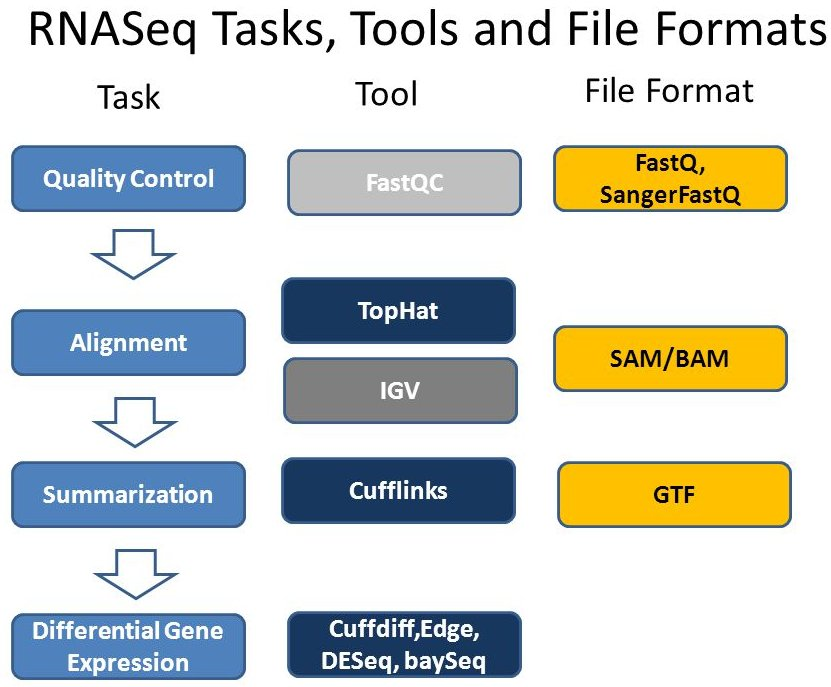
\includegraphics[width=0.8\textwidth]{c3.transcriptome/workflow.tool.format.01.jpg}
  \end{figure}
\end{frame}

\begin{frame}
  \frametitle{转录组学 | RNA-Seq | 分析 | 概览}
  \begin{figure}
    \centering
    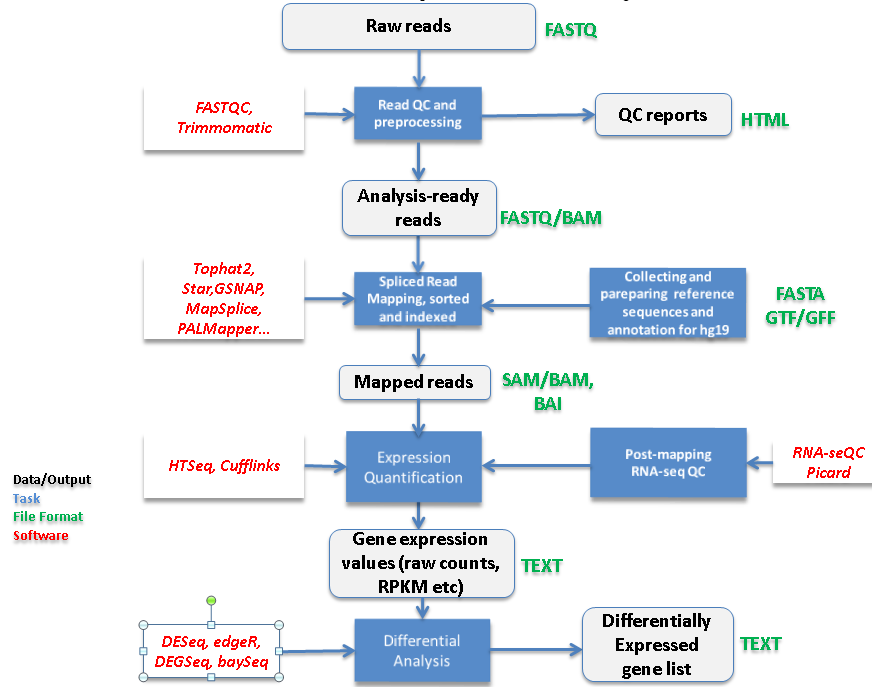
\includegraphics[width=0.8\textwidth]{c3.transcriptome/workflow.tool.format.02.png}
  \end{figure}
\end{frame}

\subsubsection{流程}
\begin{frame}
  \frametitle{转录组学 | RNA-Seq | 分析 | 流程}
  \begin{figure}
    \centering
    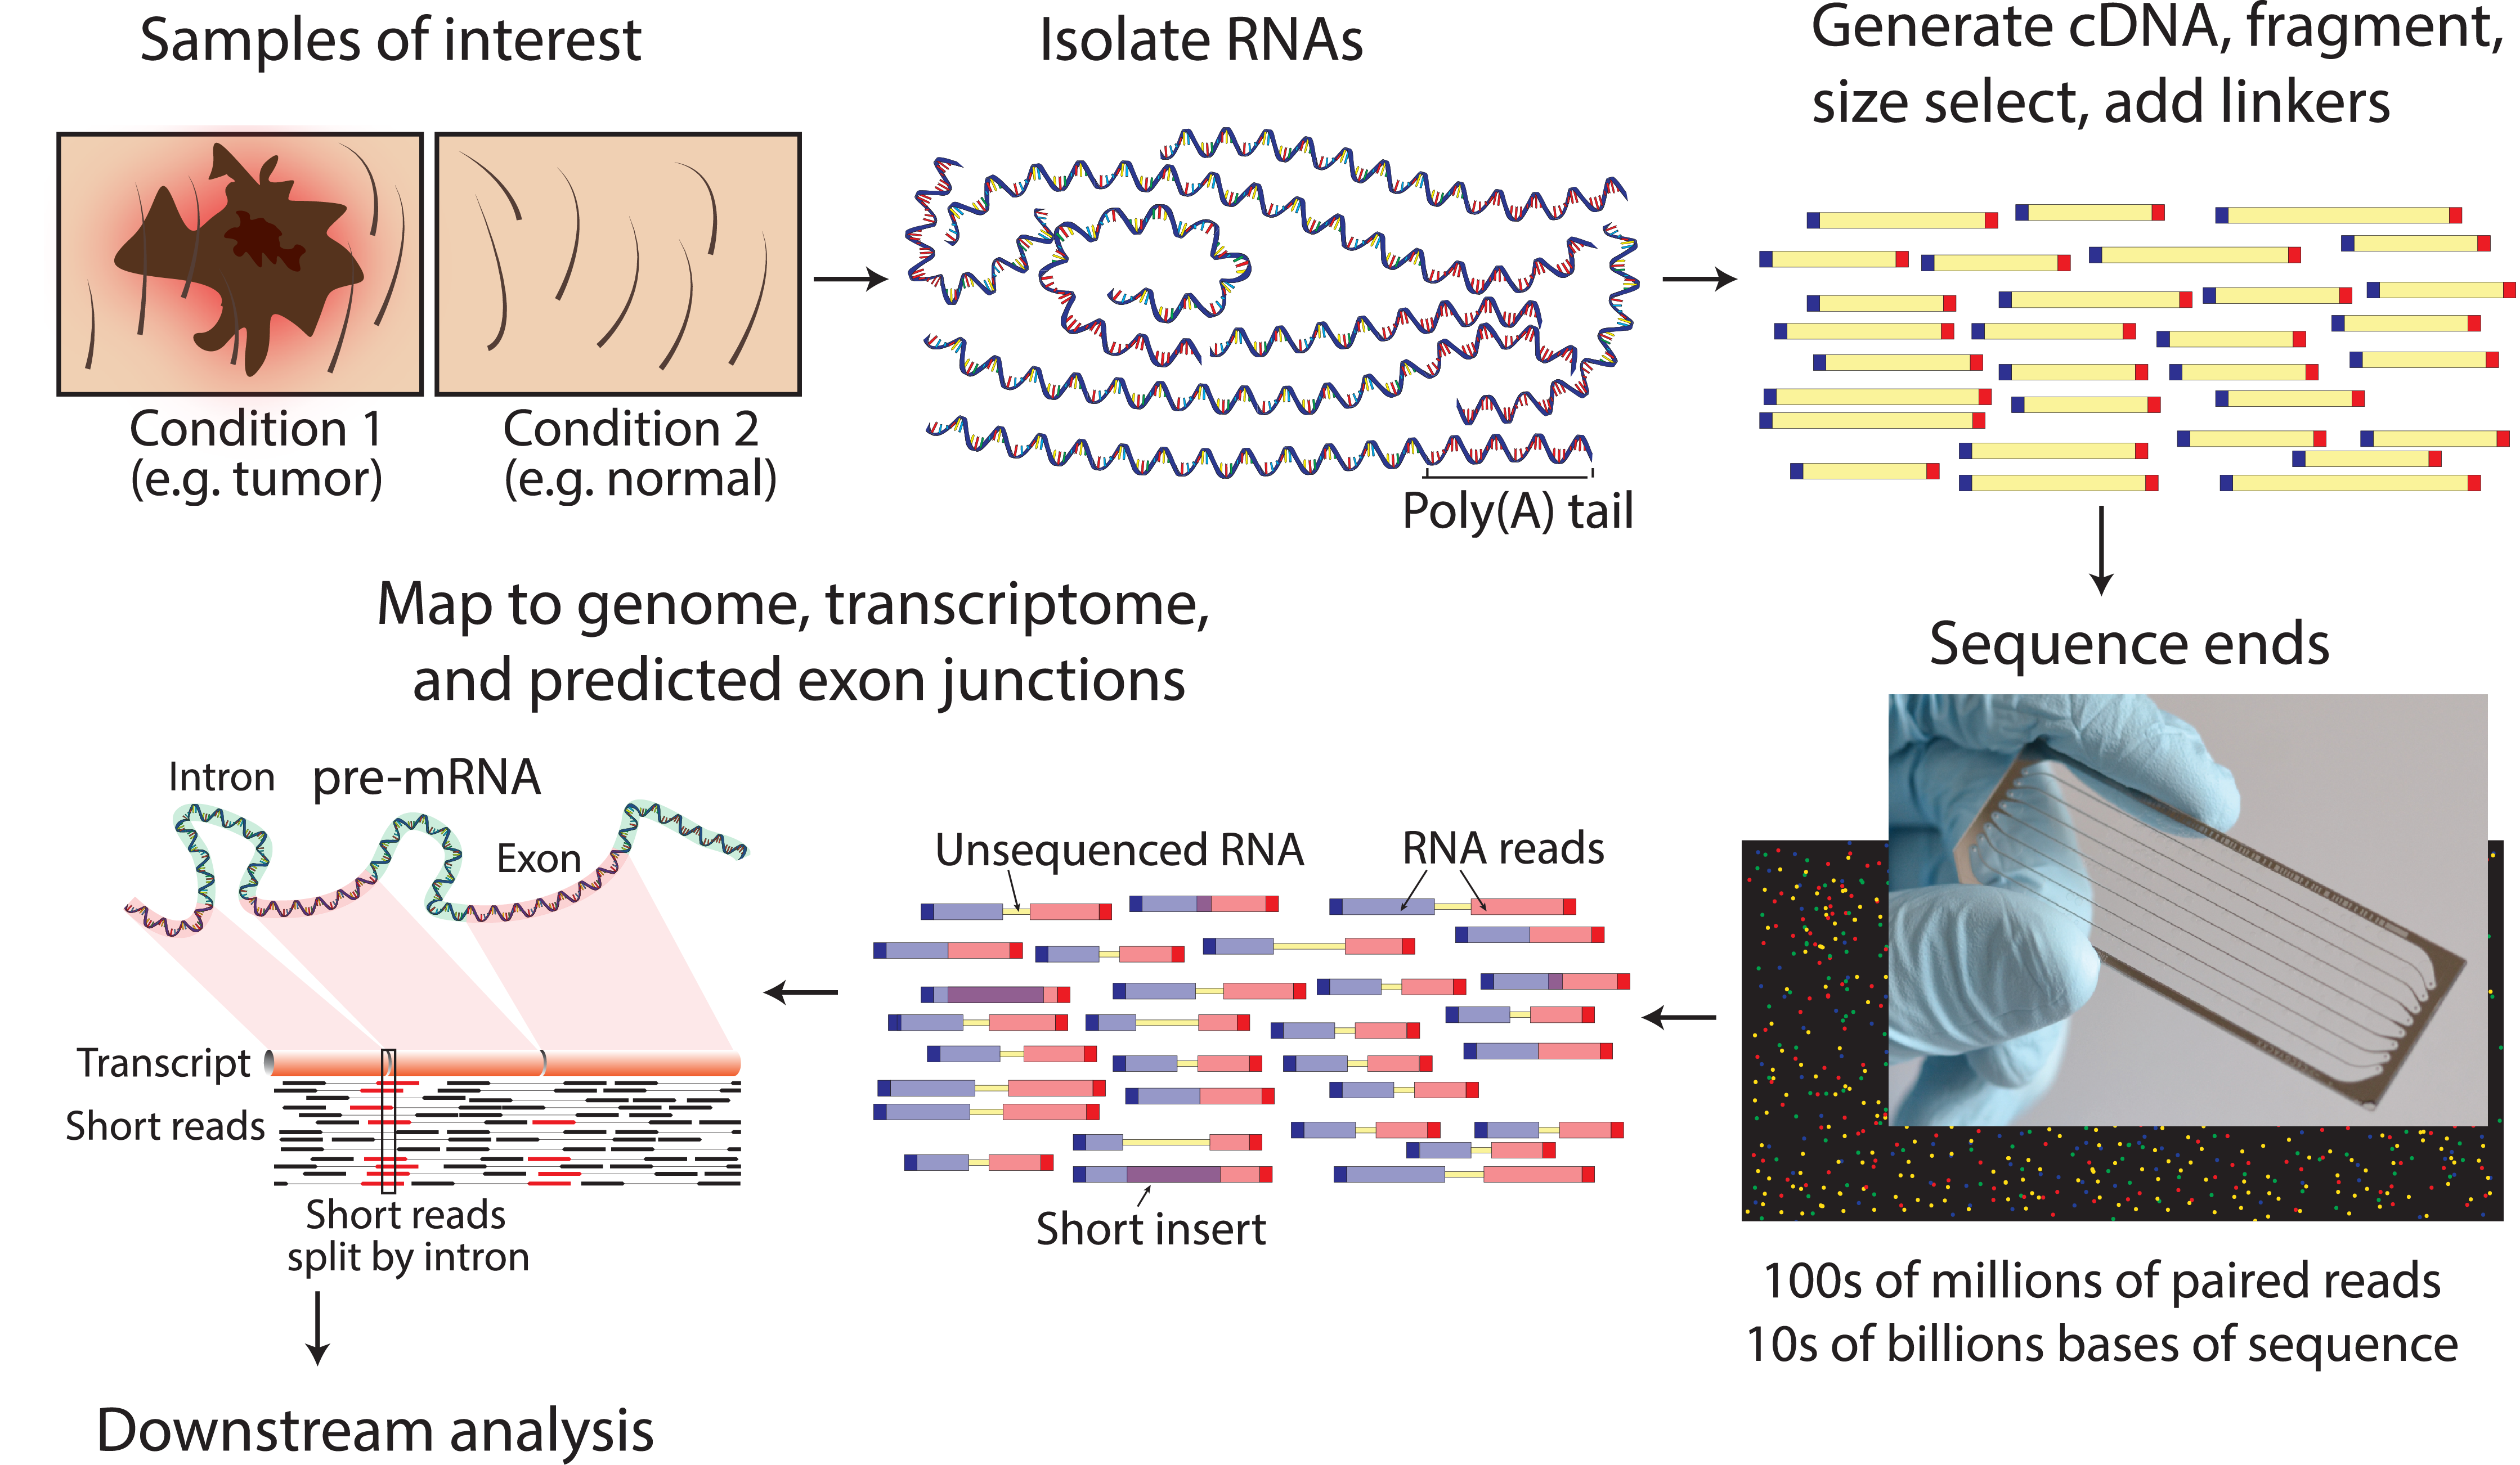
\includegraphics[width=0.9\textwidth]{c3.transcriptome/workflow.all.02.png}
  \end{figure}
\end{frame}

\begin{frame}
  \frametitle{转录组学 | RNA-Seq | 分析 | 流程}
  \begin{figure}
    \centering
    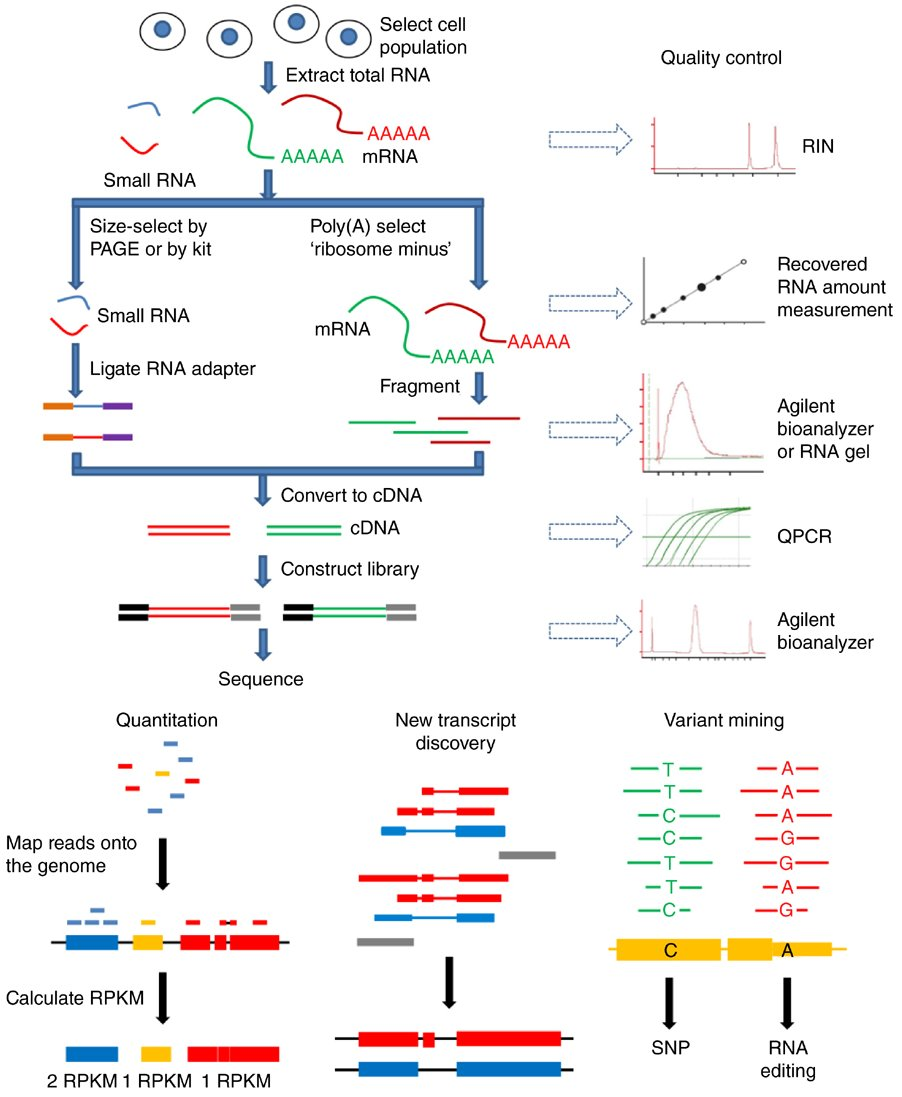
\includegraphics[width=0.53\textwidth]{c3.transcriptome/workflow.all.03.jpg}
  \end{figure}
\end{frame}

\begin{frame}
  \frametitle{转录组学 | RNA-Seq | 分析 | 流程}
  \begin{figure}
    \centering
    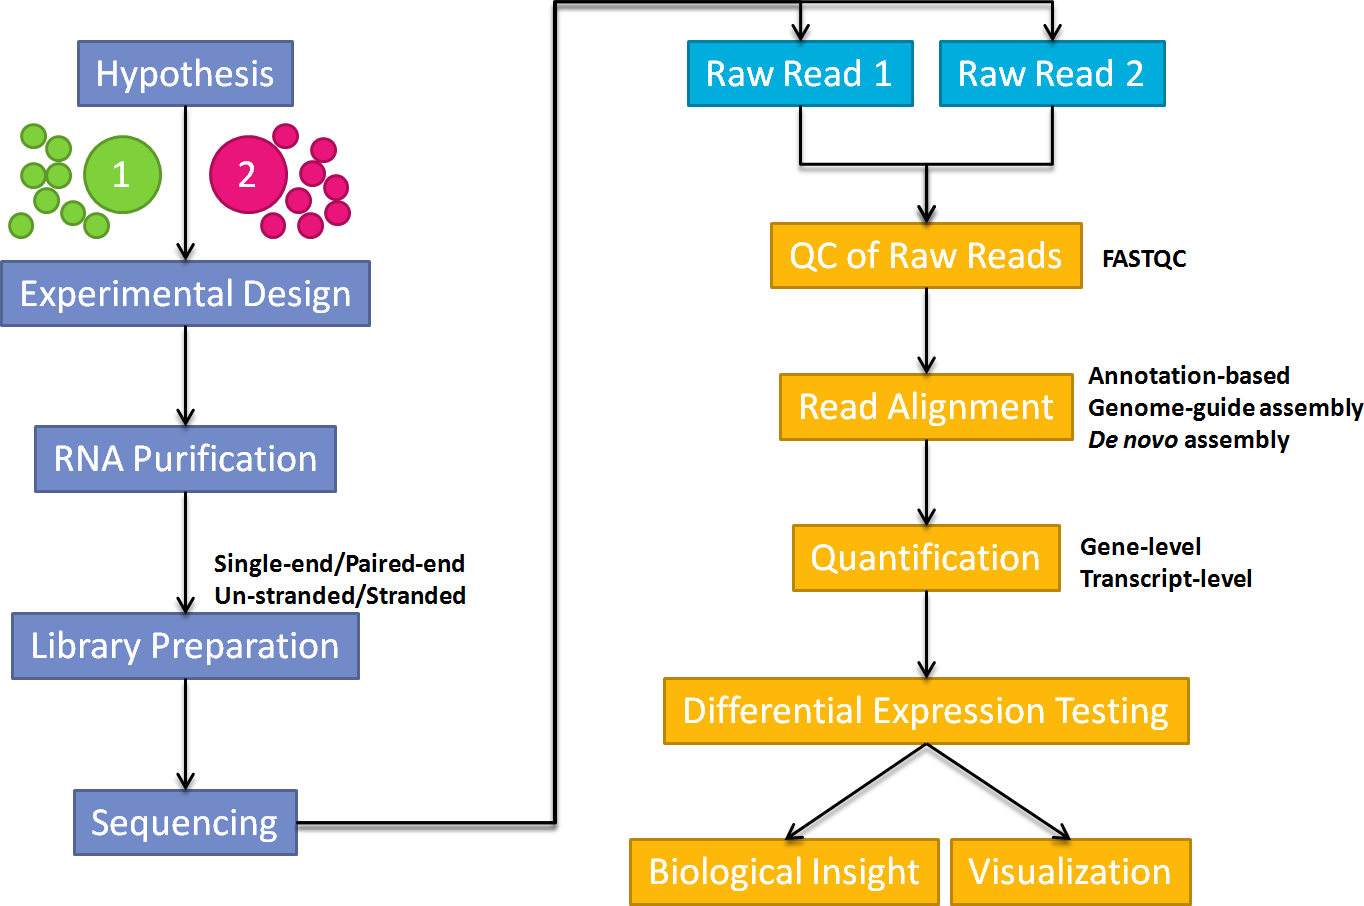
\includegraphics[width=0.9\textwidth]{c3.transcriptome/workflow.all.04.png}
  \end{figure}
\end{frame}

\begin{frame}
  \frametitle{转录组学 | RNA-Seq | 分析 | 流程 | 实验}
  \begin{figure}
    \centering
    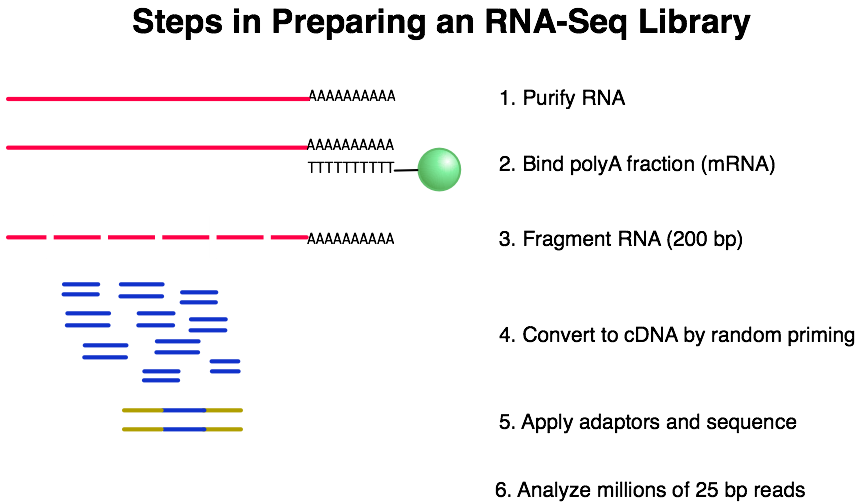
\includegraphics[width=0.9\textwidth]{c3.transcriptome/workflow.exp.01.png}
  \end{figure}
\end{frame}

\begin{frame}
  \frametitle{转录组学 | RNA-Seq | 分析 | 流程 | 实验}
  \begin{figure}
    \centering
    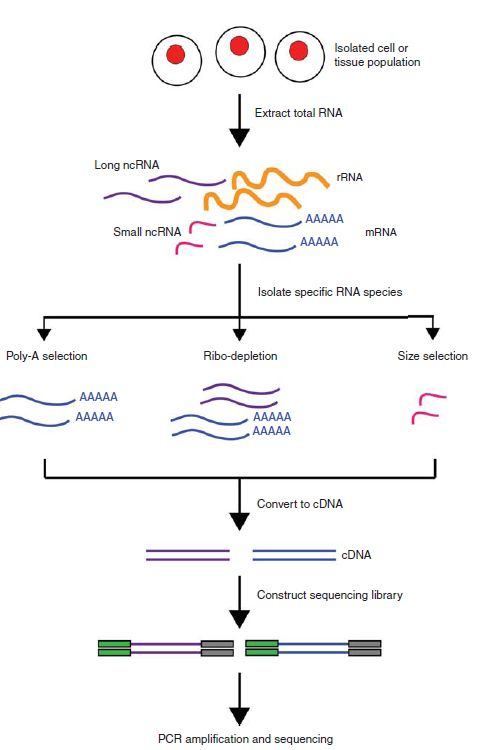
\includegraphics[width=0.4\textwidth]{c3.transcriptome/workflow.exp.02.jpg}
  \end{figure}
\end{frame}

\begin{frame}
  \frametitle{转录组学 | RNA-Seq | 分析 | 流程 | 实验}
  \begin{figure}
    \centering
    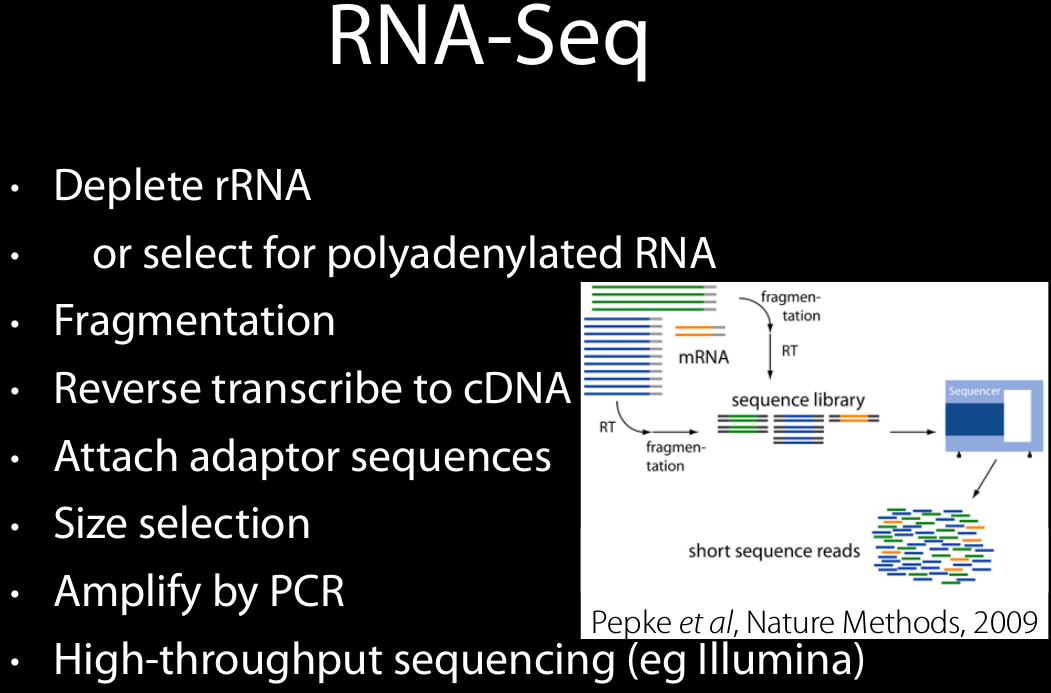
\includegraphics[width=0.9\textwidth]{c3.transcriptome/workflow.exp.03.png}
  \end{figure}
\end{frame}

\begin{frame}
  \frametitle{转录组学 | RNA-Seq | 分析 | 流程 | 实验}
  \begin{figure}
    \centering
    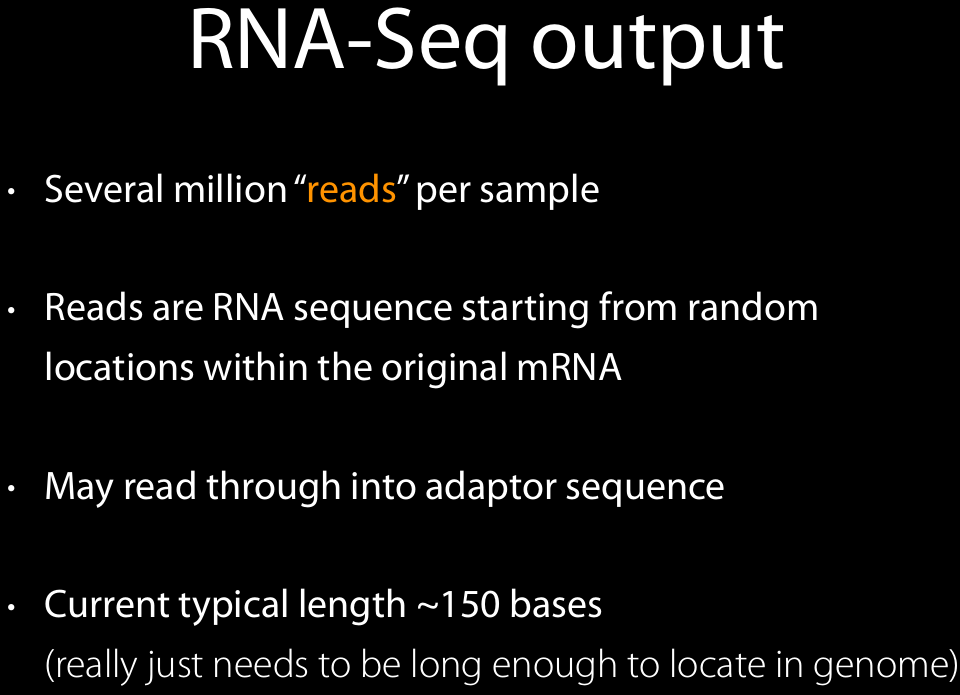
\includegraphics[width=0.85\textwidth]{c3.transcriptome/workflow.exp.04.png}
  \end{figure}
\end{frame}

\begin{frame}
  \frametitle{转录组学 | RNA-Seq | 分析 | 流程 | 生信}
  \begin{figure}
    \centering
    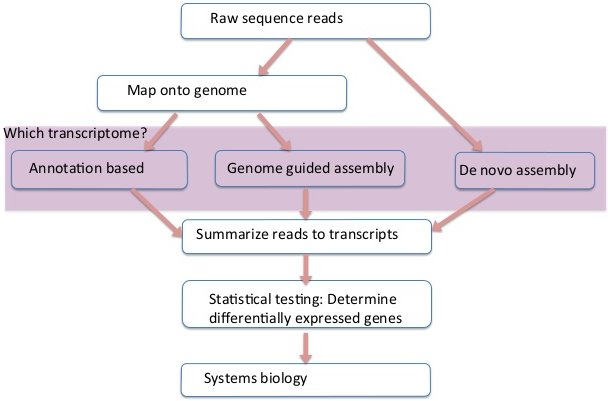
\includegraphics[width=0.9\textwidth]{c3.transcriptome/workflow.bx.01.jpg}
  \end{figure}
\end{frame}

\begin{frame}
  \frametitle{转录组学 | RNA-Seq | 分析 | 流程 | 生信}
  \begin{figure}
    \centering
    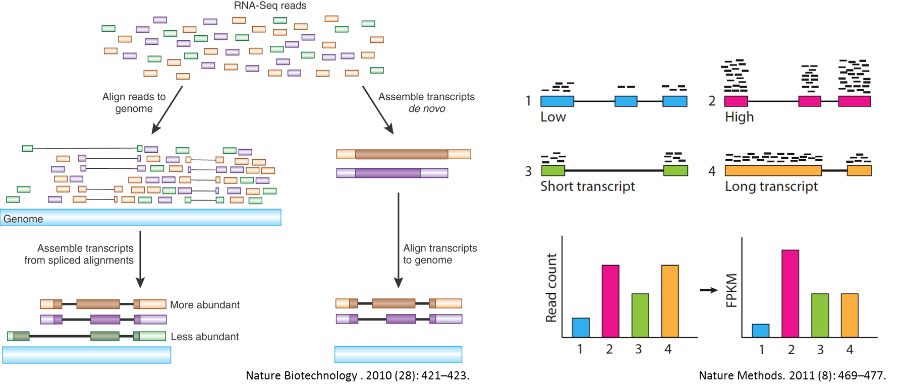
\includegraphics[width=0.9\textwidth]{c3.transcriptome/workflow.bx.02.png}
  \end{figure}
\end{frame}

\begin{frame}
  \frametitle{转录组学 | RNA-Seq | 分析 | 流程 | 生信}
  \begin{figure}
    \centering
    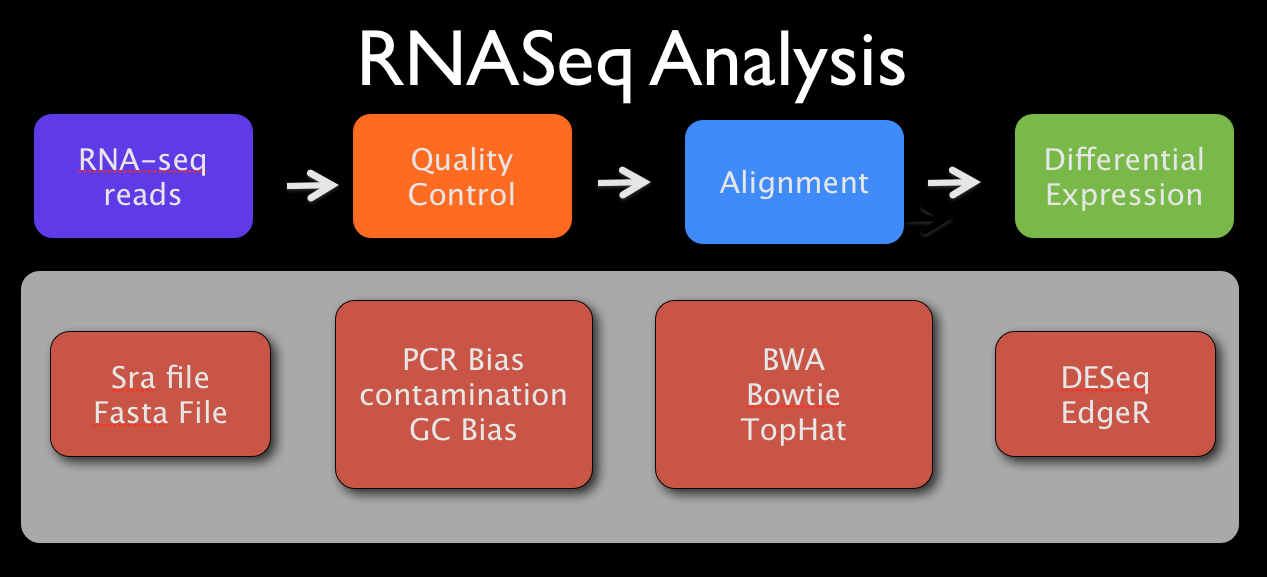
\includegraphics[width=0.7\textwidth]{c3.transcriptome/workflow.bx.03.png}\\
    \vspace{1em}
    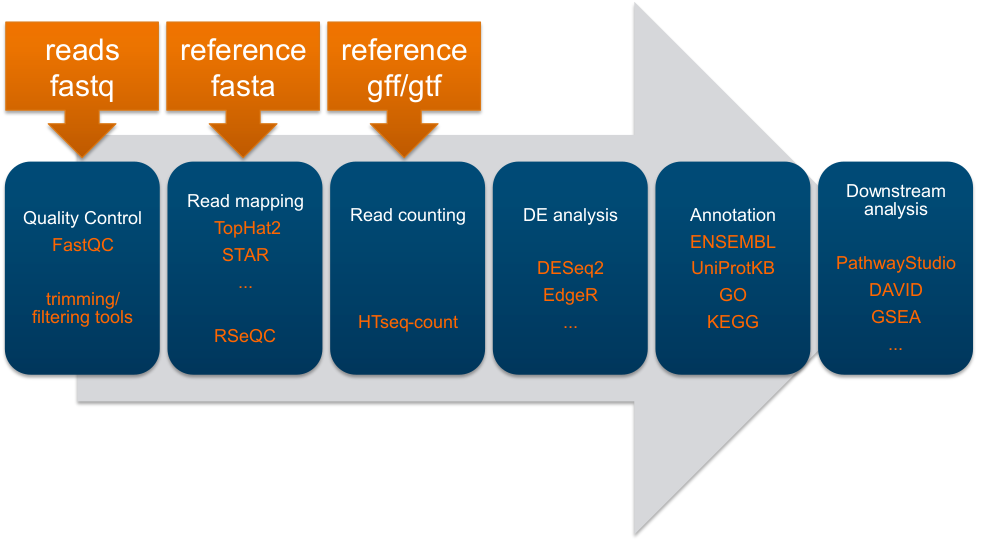
\includegraphics[width=0.7\textwidth]{c3.transcriptome/workflow.bx.30.png}
  \end{figure}
\end{frame}

\begin{frame}
  \frametitle{转录组学 | RNA-Seq | 分析 | 流程 | 生信}
  \begin{figure}
    \centering
    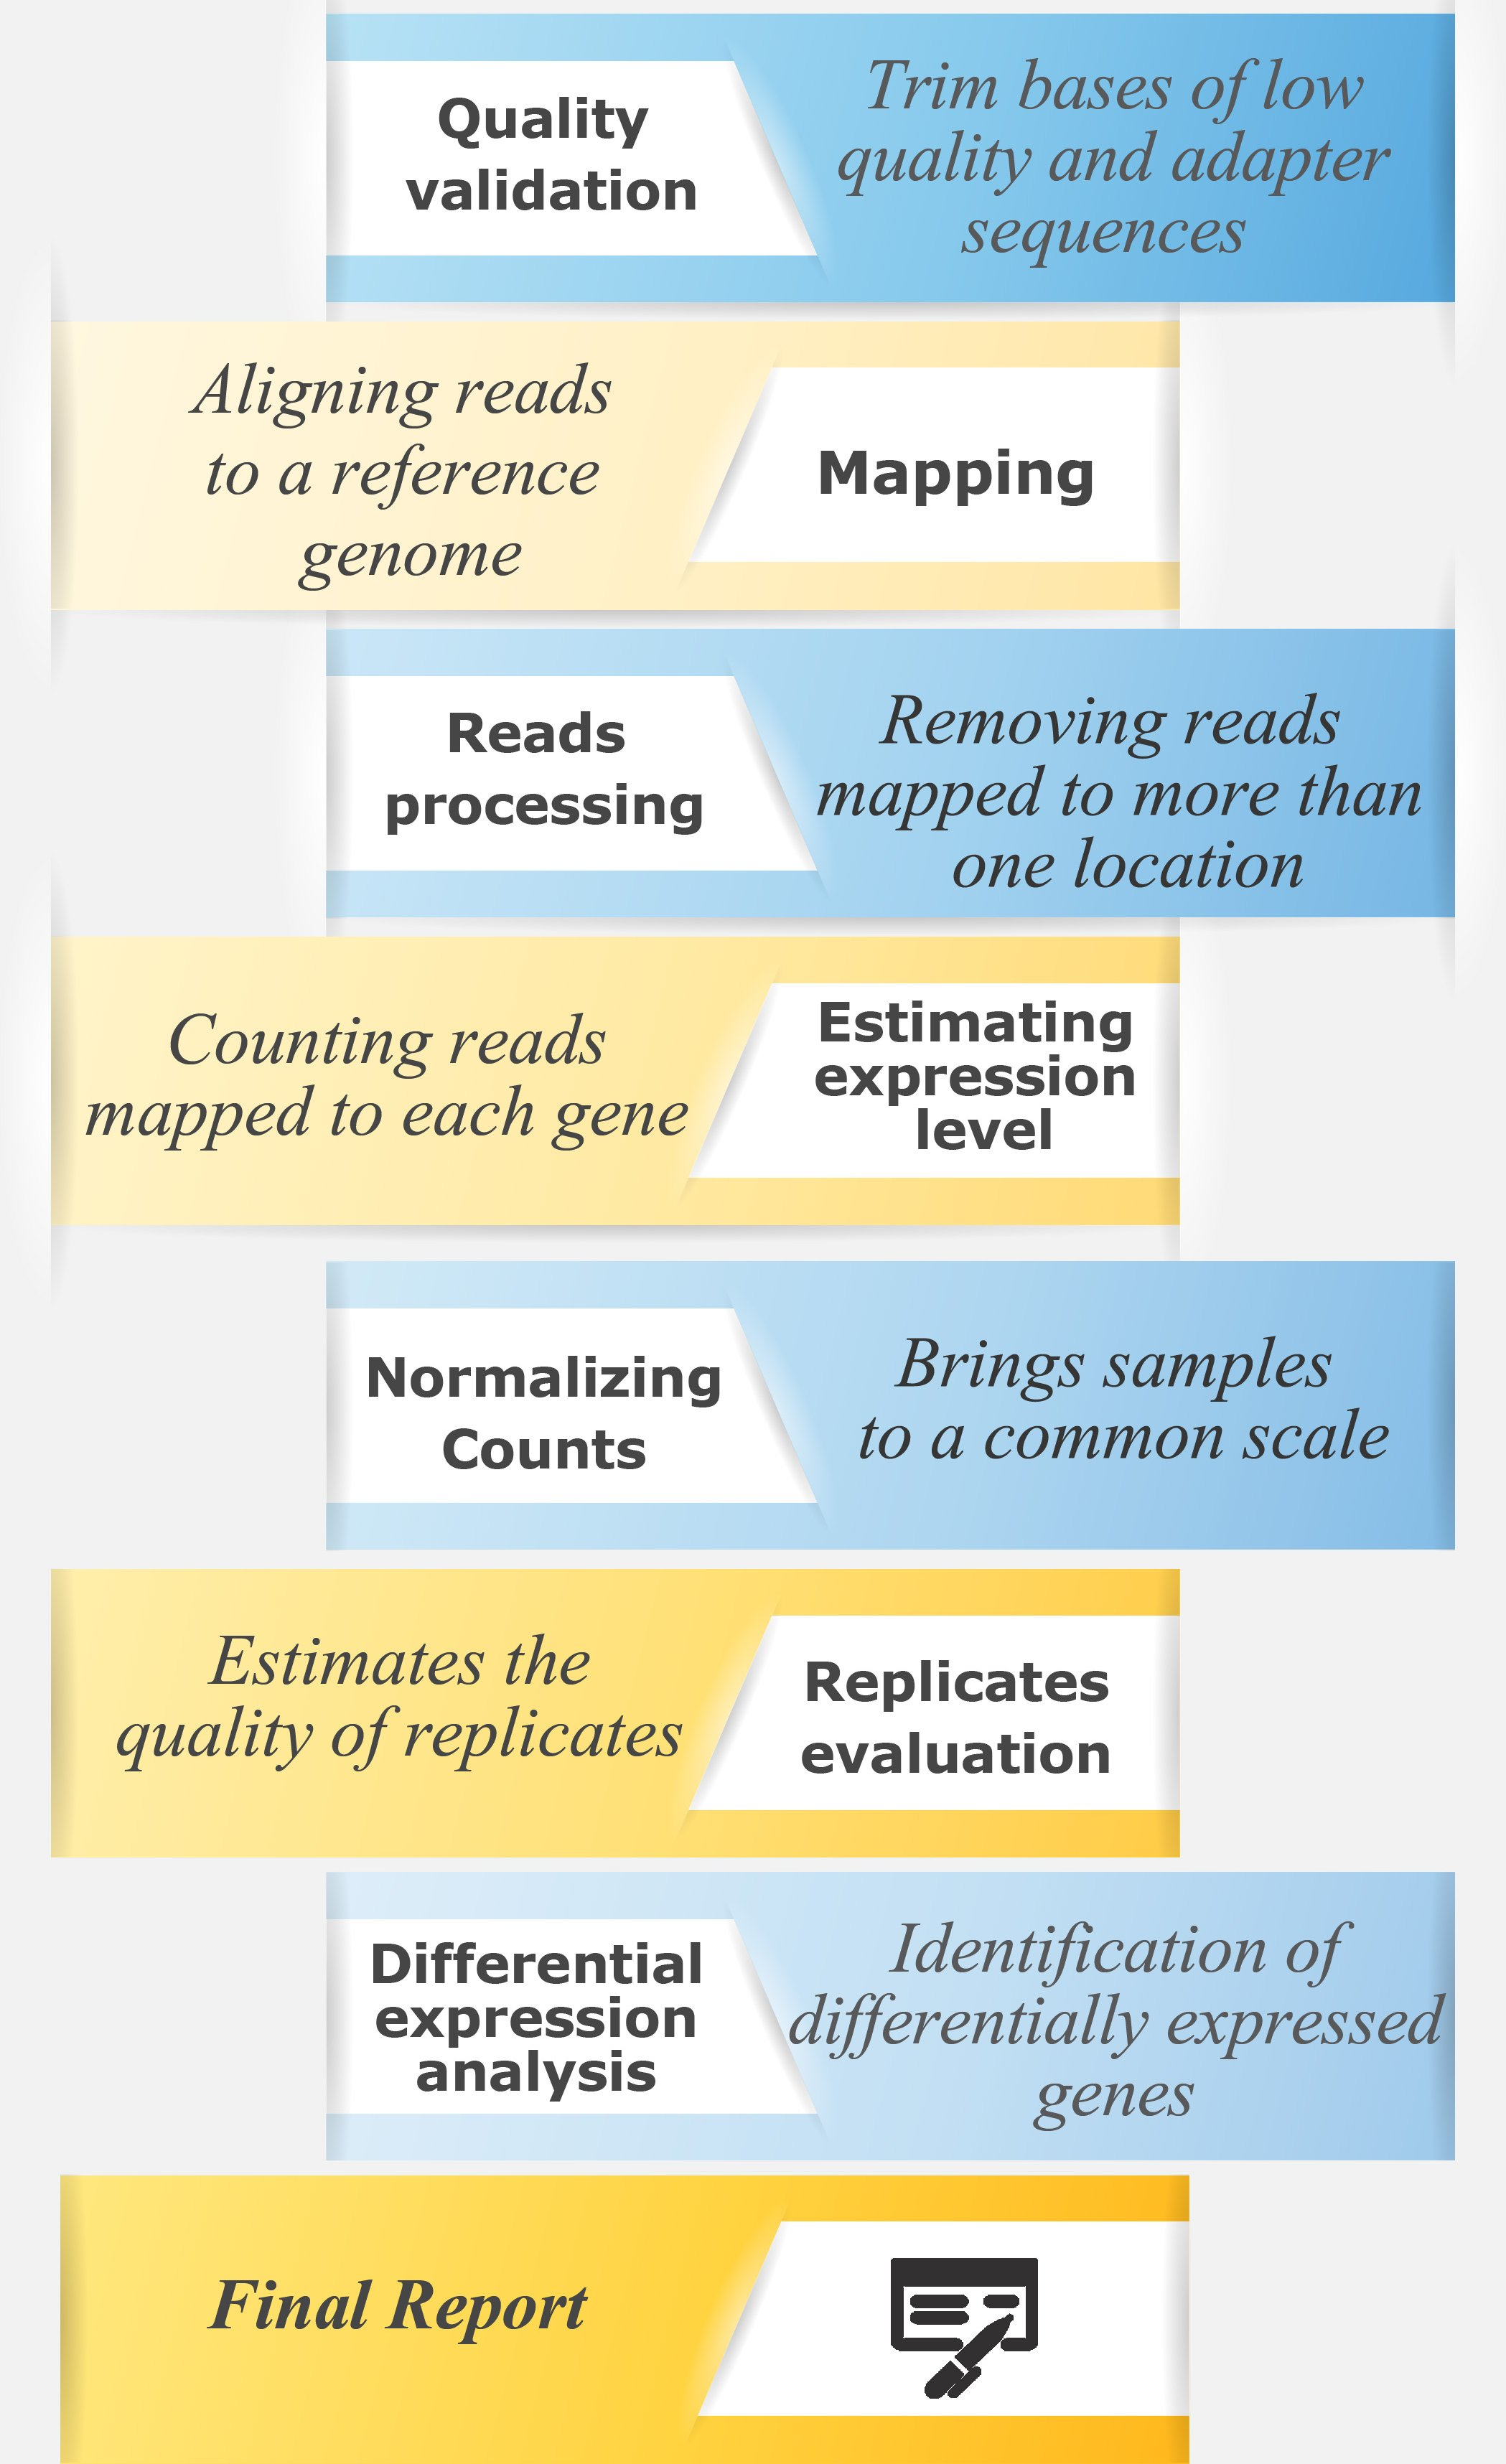
\includegraphics[width=0.4\textwidth]{c3.transcriptome/workflow.bx.04.jpg}
  \end{figure}
\end{frame}

\begin{frame}
  \frametitle{转录组学 | RNA-Seq | 分析 | 流程 | 生信}
  \begin{figure}
    \centering
    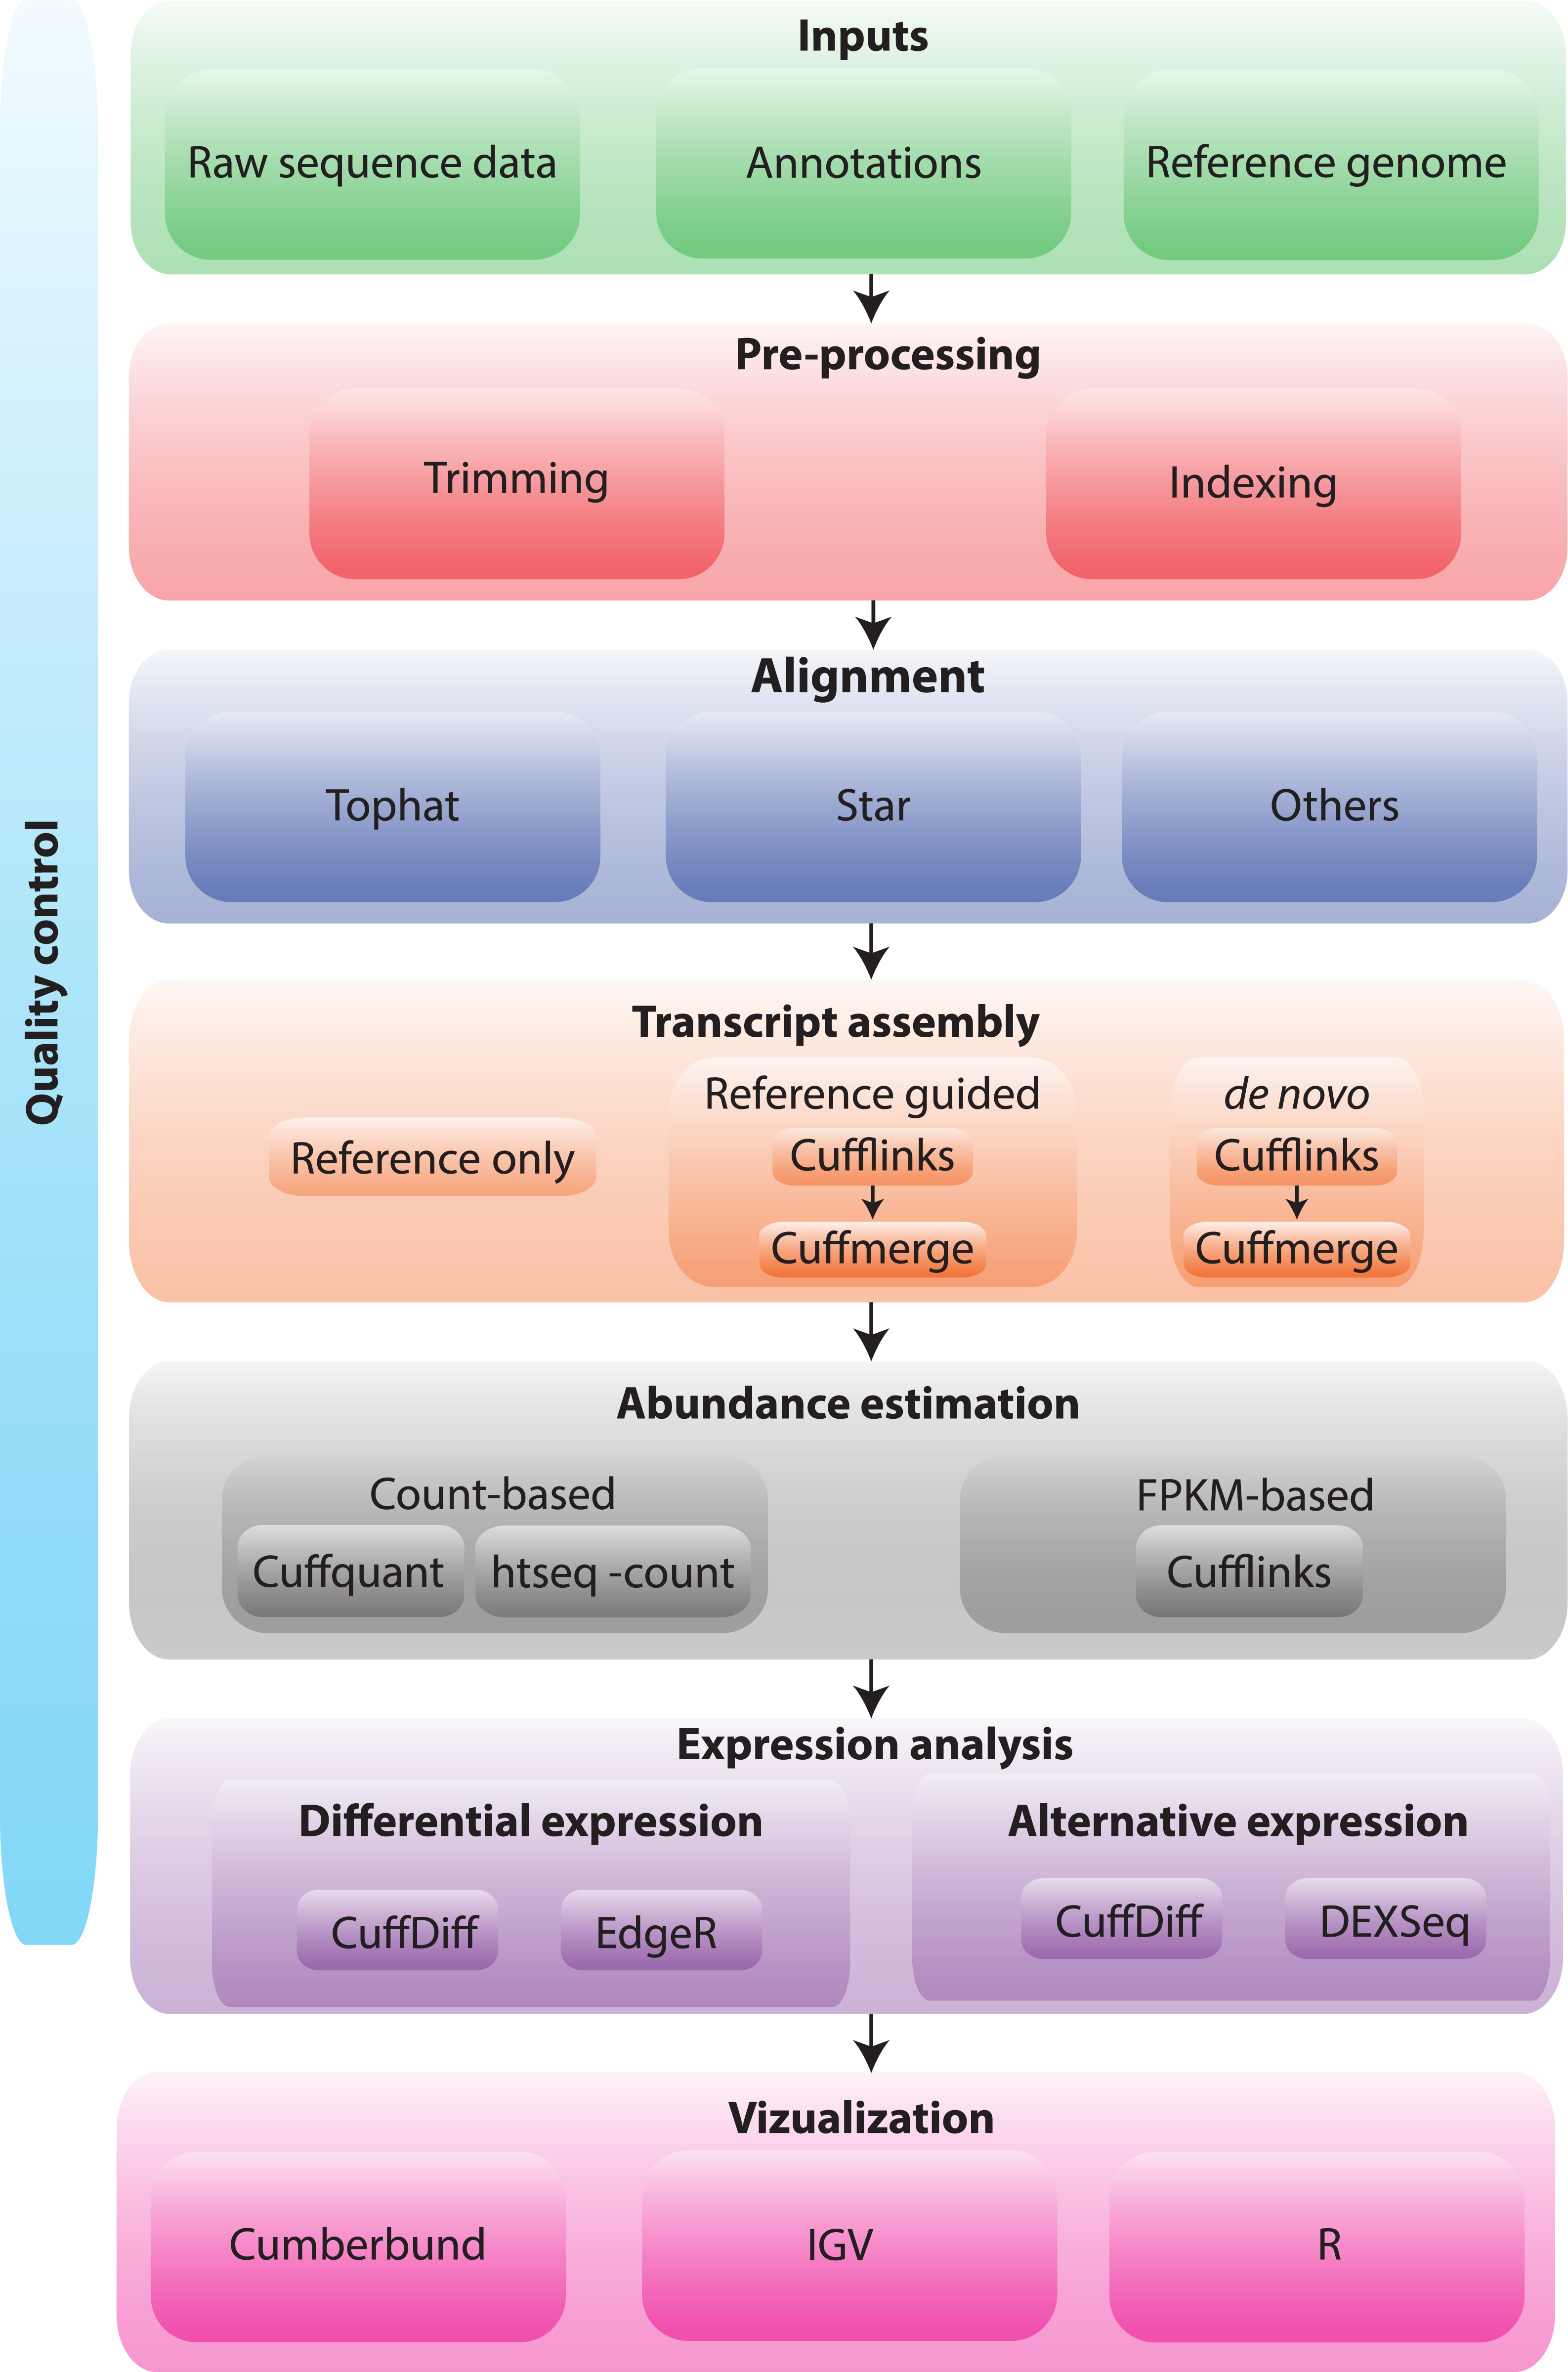
\includegraphics[width=0.4\textwidth]{c3.transcriptome/workflow.bx.05.png}
  \end{figure}
\end{frame}

\begin{frame}
  \frametitle{转录组学 | RNA-Seq | 分析 | 流程 | 生信}
  \begin{figure}
    \centering
    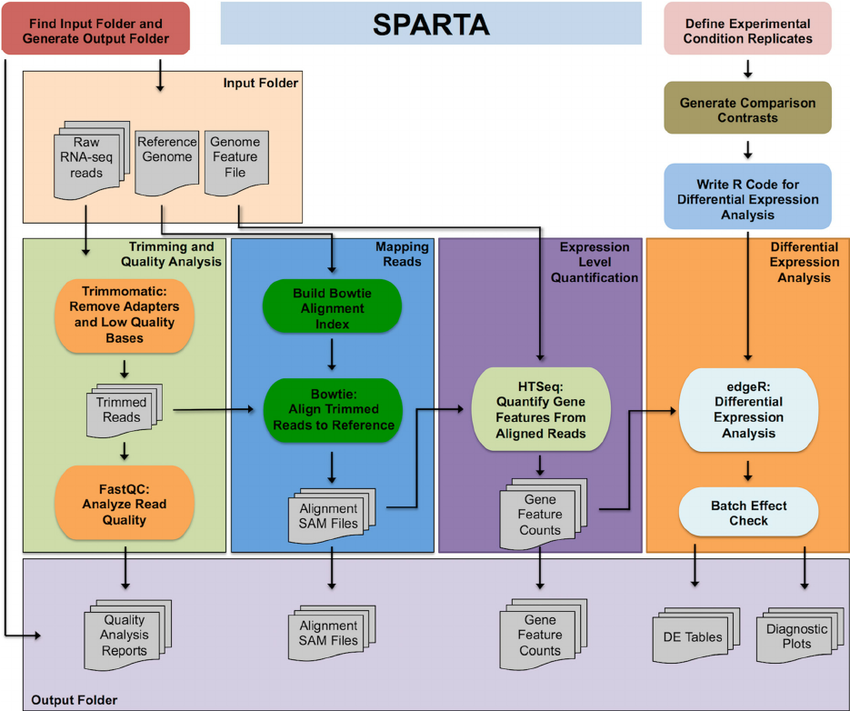
\includegraphics[width=0.7\textwidth]{c3.transcriptome/workflow.bx.06.png}
  \end{figure}
\end{frame}

\begin{frame}
  \frametitle{转录组学 | RNA-Seq | 分析 | 流程 | 生信}
  \begin{figure}
    \centering
    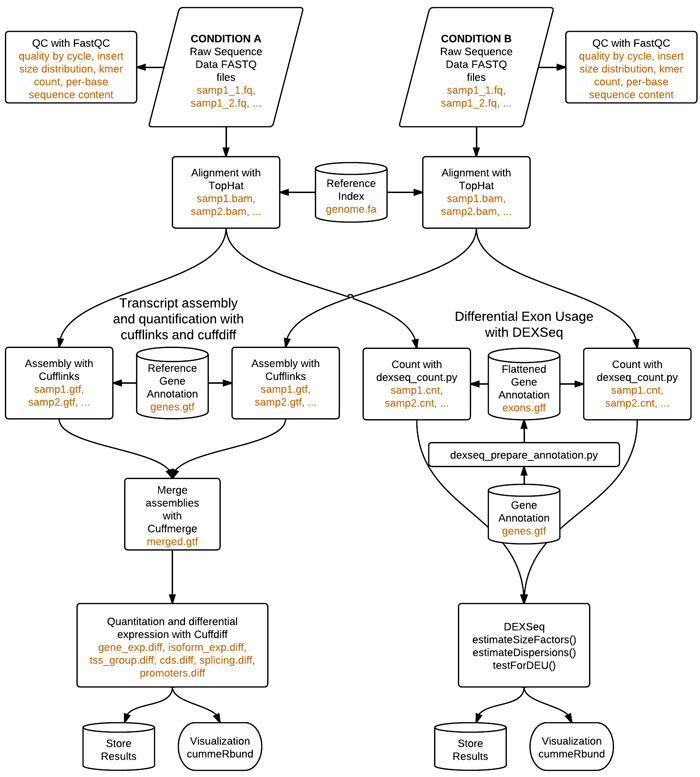
\includegraphics[width=0.6\textwidth]{c3.transcriptome/workflow.bx.07.png}
  \end{figure}
\end{frame}

\begin{frame}
  \frametitle{转录组学 | RNA-Seq | 分析 | 流程 | 生信}
  \begin{figure}
    \centering
    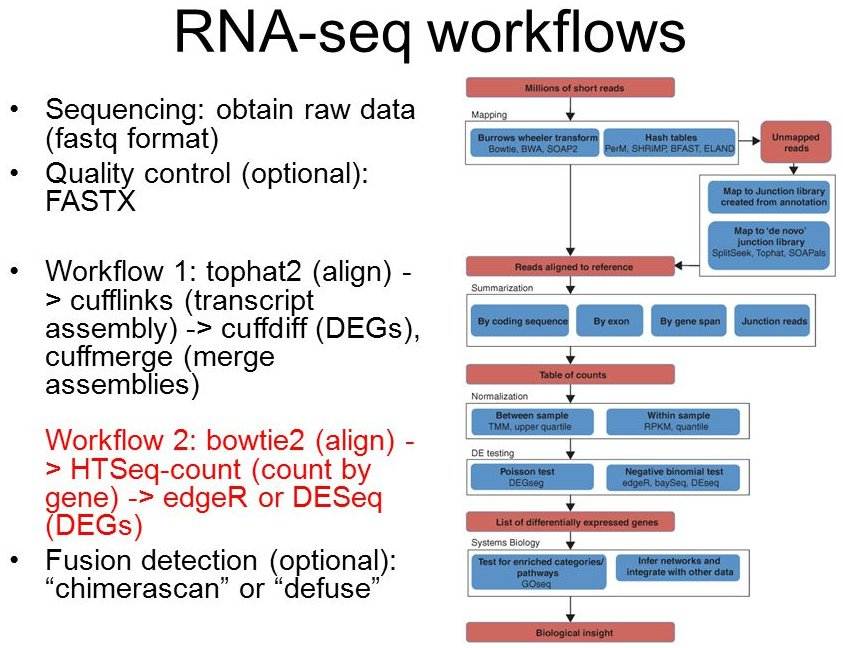
\includegraphics[width=0.8\textwidth]{c3.transcriptome/workflow.bx.08.jpg}
  \end{figure}
\end{frame}

\begin{frame}
  \frametitle{转录组学 | RNA-Seq | 分析 | 流程 | 补遗 | Single cell}
  \begin{figure}
    \centering
    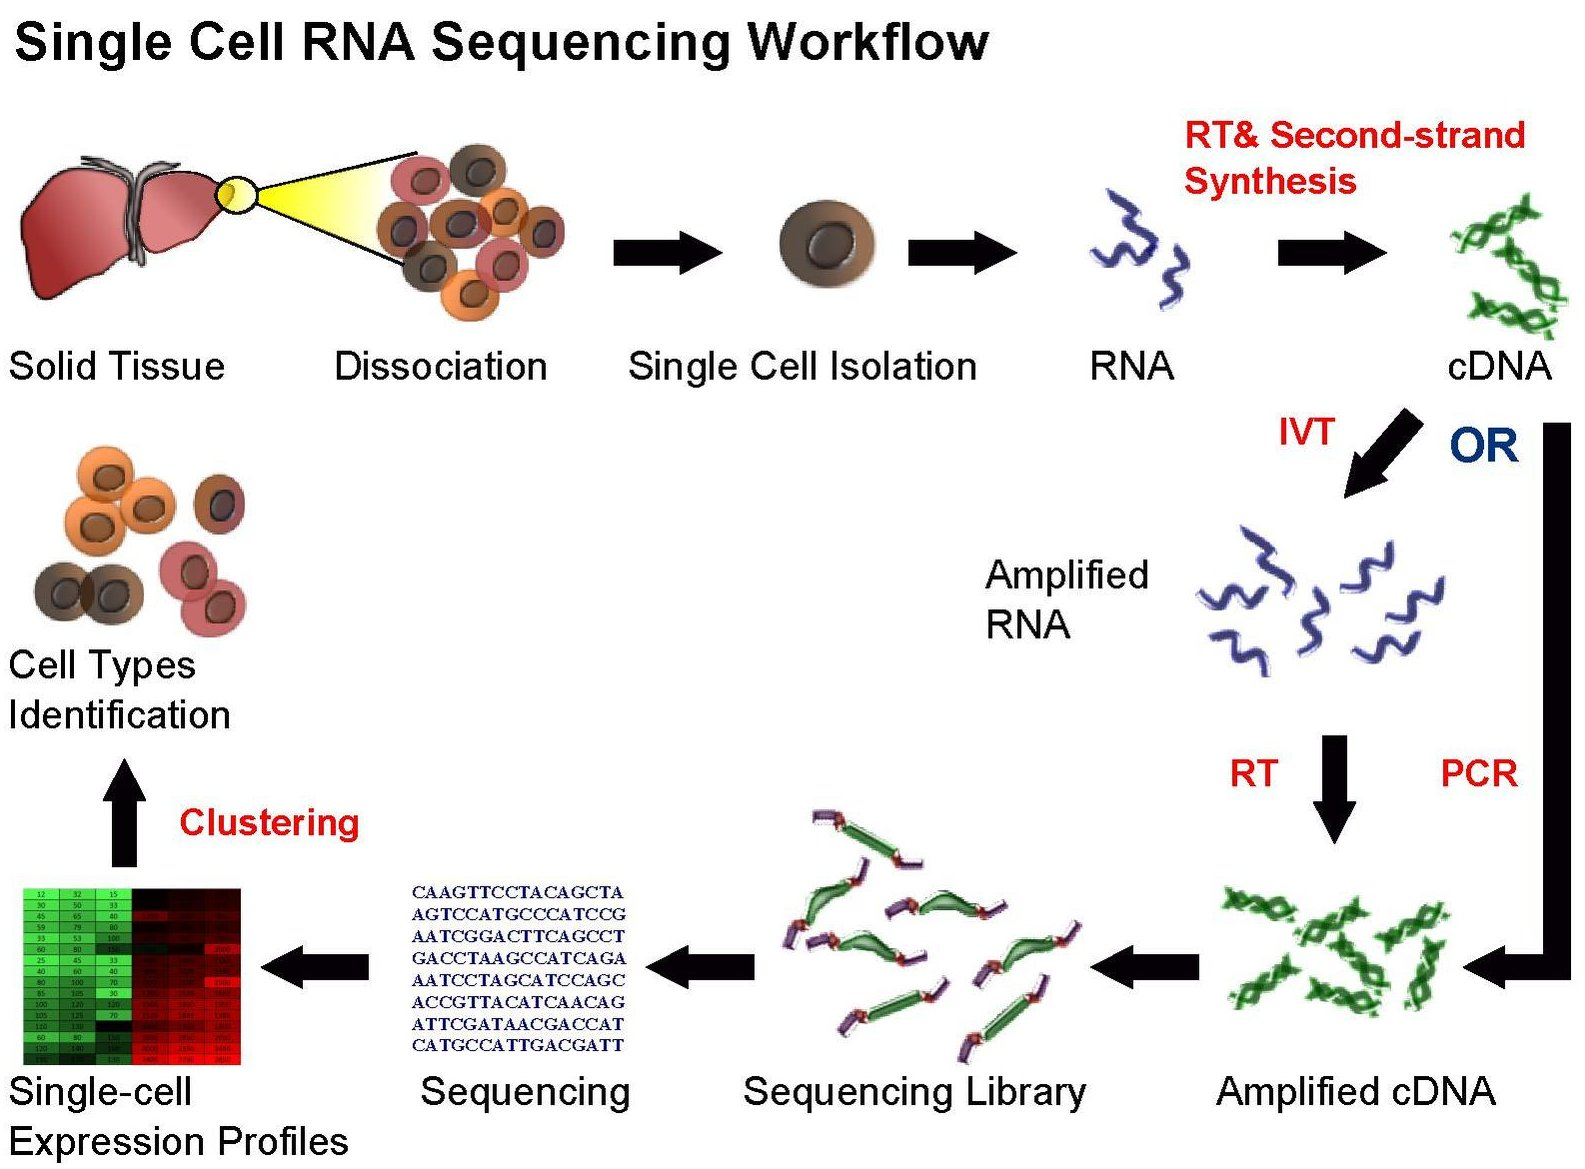
\includegraphics[width=0.85\textwidth]{c3.transcriptome/workflow.single.cell.01.jpg}
  \end{figure}
\end{frame}

\begin{frame}
  \frametitle{转录组学 | RNA-Seq | 分析 | 流程 | 补遗 | Stranded}
  \begin{figure}
    \centering
    \includegraphics[width=0.55\textwidth]{c3.transcriptome/workflow.strand.01.jpg}
  \end{figure}
\end{frame}

\begin{frame}
  \frametitle{转录组学 | RNA-Seq | 分析 | 流程 | 补遗 | Stranded}
  \begin{figure}
    \centering
    \includegraphics[width=0.9\textwidth]{c3.transcriptome/workflow.strand.02.png}
  \end{figure}
\end{frame}

\begin{frame}
  \frametitle{转录组学 | RNA-Seq | 分析 | 流程 | 补遗 | miRNA}
  \begin{figure}
    \centering
    \includegraphics[width=0.9\textwidth]{c3.transcriptome/workflow.mirna.01.jpg}
  \end{figure}
\end{frame}

\begin{frame}
  \frametitle{转录组学 | RNA-Seq | 分析 | 流程 | 补遗 | miRNA}
  \begin{figure}
    \centering
    \includegraphics[width=0.55\textwidth]{c3.transcriptome/workflow.mirna.02.png}
  \end{figure}
\end{frame}

\begin{frame}
  \frametitle{转录组学 | RNA-Seq | 分析 | 流程 | 补遗 | miRNA}
  \begin{figure}
    \centering
    \includegraphics[width=0.48\textwidth]{c3.transcriptome/workflow.mirna.03.png}
  \end{figure}
\end{frame}

\subsubsection{术语}
\begin{frame}
  \frametitle{转录组学 | RNA-Seq | 分析 | 术语 | 引言}
  \begin{figure}
    \centering
    \includegraphics[width=0.9\textwidth]{c3.transcriptome/term.count.01.png}
  \end{figure}
\end{frame}

\begin{frame}
  \frametitle{转录组学 | RNA-Seq | 分析 | 术语 | 引言}
  \begin{figure}
    \centering
    \includegraphics[width=0.8\textwidth]{c3.transcriptome/term.count.02.png}
  \end{figure}
\end{frame}

\begin{frame}
  \frametitle{转录组学 | RNA-Seq | 分析 | 术语 | 引言}
  \begin{figure}
    \centering
    \includegraphics[width=0.9\textwidth]{c3.transcriptome/term.all.01.jpg}
  \end{figure}
\end{frame}

\begin{frame}
  \frametitle{转录组学 | RNA-Seq | 分析 | 术语 | 引言}
  \begin{figure}
    \centering
    \includegraphics[width=0.9\textwidth]{c3.transcriptome/term.norm.01.png}
  \end{figure}
\end{frame}

\begin{frame}
  \frametitle{转录组学 | RNA-Seq | 分析 | 术语 | 引言}
  \begin{figure}
    \centering
    \includegraphics[width=0.9\textwidth]{c3.transcriptome/term.norm.02.png}
  \end{figure}
\end{frame}

\begin{frame}
  \frametitle{转录组学 | RNA-Seq | 分析 | 术语 | 引言}
  \begin{figure}
    \centering
    \includegraphics[width=0.9\textwidth]{c3.transcriptome/term.norm.03.png}
  \end{figure}
\end{frame}

\begin{frame}
  \frametitle{转录组学 | RNA-Seq | 分析 | 术语 | 引言}
  \begin{figure}
    \centering
    \includegraphics[width=0.9\textwidth]{c3.transcriptome/term.norm.04.png}
  \end{figure}
\end{frame}

\begin{frame}
  \frametitle{转录组学 | RNA-Seq | 分析 | 术语 | 引言}
  \begin{figure}
    \centering
    \includegraphics[width=\textwidth]{c3.transcriptome/term.norm.06.png}
  \end{figure}
\end{frame}

\begin{frame}
  \frametitle{转录组学 | RNA-Seq | 分析 | 术语 | 引言}
  \begin{figure}
    \centering
    \includegraphics[width=0.9\textwidth]{c3.transcriptome/term.all.02.jpg}
  \end{figure}
\end{frame}

\begin{frame}
  \frametitle{转录组学 | RNA-Seq | 分析 | 术语 | 引言}
  \begin{figure}
    \centering
    \includegraphics[width=0.8\textwidth]{c3.transcriptome/term.all.03.jpg}
  \end{figure}
\end{frame}

\begin{frame}
  \frametitle{转录组学 | RNA-Seq | 分析 | 术语 | 引言}
  \begin{figure}
    \centering
    \includegraphics[width=0.9\textwidth]{c3.transcriptome/term.all.04.jpg}
  \end{figure}
\end{frame}

\begin{frame}
  \frametitle{转录组学 | RNA-Seq | 分析 | 术语 | RPKM}
  \begin{figure}
    \centering
    \includegraphics[width=0.8\textwidth]{c3.transcriptome/term.rpkm.01.jpg}\\
    \vspace{1em}
    \includegraphics[width=0.7\textwidth]{c3.transcriptome/term.rpkm.02.jpg}
  \end{figure}
\end{frame}

\begin{frame}
  \frametitle{转录组学 | RNA-Seq | 分析 | 术语 | RPKM}
  \begin{figure}
    \centering
    \includegraphics[width=0.9\textwidth]{c3.transcriptome/term.rpkm.03.png}
  \end{figure}
\end{frame}

\begin{frame}
  \frametitle{转录组学 | RNA-Seq | 分析 | 术语 | FPKM}
  \begin{figure}
    \centering
    \includegraphics[width=0.9\textwidth]{c3.transcriptome/term.fpkm.01.jpg}
  \end{figure}
\end{frame}

\begin{frame}
  \frametitle{转录组学 | RNA-Seq | 分析 | 术语 | FPKM}
  \begin{figure}
    \centering
    \includegraphics[width=0.8\textwidth]{c3.transcriptome/term.fpkm.02.jpg}\\
    \vspace{1em}
    \includegraphics[width=0.6\textwidth]{c3.transcriptome/term.fpkm.03.png}
  \end{figure}
\end{frame}

\begin{frame}
  \frametitle{转录组学 | RNA-Seq | 分析 | 术语 | TPM}
  \begin{block}{TPM}
    当我们进行RNA-Seq时,会使用RPKM或者FPKM来代表某个gene或是isoform的表达量多寡。可是当我们想要比较不同次实验内的某个基因,其表达量相比于“整体基因表达”而言,是否维持在“固定比例”时,便无法使用这样的计算方式。因此Wagner \textit{et. al.}在2012年的时候提出TPM(Transcript Per Million)的概念来弥补这个缺点。
  \end{block}
\end{frame}

\begin{frame}
  \frametitle{转录组学 | RNA-Seq | 分析 | 术语 | TPM}
  \begin{figure}
    \centering
    \includegraphics[width=0.7\textwidth]{c3.transcriptome/term.tpm.01.jpg}\\
    \includegraphics[width=0.7\textwidth]{c3.transcriptome/term.tpm.02.png}\\
    \includegraphics[width=0.3\textwidth]{c3.transcriptome/term.tpm.03.png}
  \end{figure}
\end{frame}

\begin{frame}
  \frametitle{转录组学 | RNA-Seq | 分析 | 术语 | TPM}
  \begin{figure}
    \centering
    \includegraphics[width=0.9\textwidth]{c3.transcriptome/term.tpm.20.png}
  \end{figure}
\end{frame}

\begin{frame}
  \frametitle{转录组学 | RNA-Seq | 分析 | 术语 | TPM}
  \begin{figure}
    \centering
    \includegraphics[width=0.75\textwidth]{c3.transcriptome/term.tpm.21.png}
  \end{figure}
\end{frame}

\begin{frame}
  \frametitle{转录组学 | RNA-Seq | 分析 | 术语 | TPM}
  \begin{figure}
    \centering
    \includegraphics[width=0.65\textwidth]{c3.transcriptome/term.tpm.22.png}
  \end{figure}
\end{frame}

\begin{frame}
  \frametitle{转录组学 | RNA-Seq | 分析 | 术语 | TPM}
  \begin{block}{比较}
比较RPKM和TPM的表格之后,可以发现RPKM在“Sum”这一行,三个实验中的数值均不同,因此我们很难直接利用RPKM数值去比较每个基因“相对于整体”的表达量多寡。然而TMP则一律为1,000,000,也就是1 million,意即TPM的定义(Transcript \textbf{Per Million})。因此这些数值便可以直接比较,了解基因之间的相对表达量。
  \end{block}
\end{frame}

\begin{frame}
  \frametitle{转录组学 | RNA-Seq | 分析 | 术语 | 总结}
  \begin{block}{Metrics}
    \begin{itemize}
      \item RPKM (Reads Per Kilobase Million)
      \item FPKM (Fragments Per Kilobase Million)
      \item TPM (Transcripts Per Kilobase Million)
    \end{itemize}
        These three metrics attempt to normalize for sequencing depth and gene length. 
  \end{block}
\end{frame}

\begin{frame}
  \frametitle{转录组学 | RNA-Seq | 分析 | 术语 | 总结}
  \begin{block}{RPKM}
    Here's how you do it for RPKM:
    \begin{enumerate}
      \item Count up the total reads in a sample and divide that number by 1,000,000 –\ this is our ``per million" scaling factor.
      \item Divide the read counts by the ``per million" scaling factor. This normalizes for sequencing depth, giving you reads per million (RPM)
      \item Divide the RPM values by the length of the gene, in kilobases. This gives you RPKM.
    \end{enumerate}
  \end{block}
\end{frame}

\begin{frame}
  \frametitle{转录组学 | RNA-Seq | 分析 | 术语 | 总结}
  \begin{block}{FPKM}
 FPKM is very similar to RPKM. RPKM was made for single-end RNA-seq, where every read corresponded to a single fragment that was sequenced. FPKM was made for paired-end RNA-seq. With paired-end RNA-seq, two reads can correspond to a single fragment, or, if one read in the pair did not map, one read can correspond to a single fragment. The only difference between RPKM and FPKM is that FPKM takes into account that two reads can map to one fragment (and so it doesn't count this fragment twice). 
  \end{block}
\end{frame}

\begin{frame}
  \frametitle{转录组学 | RNA-Seq | 分析 | 术语 | 总结}
  \begin{block}{TPM}
    TPM is very similar to RPKM and FPKM. The only difference is the order of operations. Here's how you calculate TPM:
    \begin{enumerate}
      \item Divide the read counts by the length of each gene in kilobases. This gives you reads per kilobase (RPK).
      \item Count up all the RPK values in a sample and divide this number by 1,000,000. This is your ``per million" scaling factor.
      \item Divide the RPK values by the ``per million" scaling factor. This gives you TPM.
    \end{enumerate}
    So you see, when calculating TPM, the only difference is that you normalize for gene length first, and then normalize for sequencing depth second. However, the effects of this difference are quite profound.
  \end{block}
\end{frame}

\begin{frame}
  \frametitle{转录组学 | RNA-Seq | 分析 | 术语 | 总结}
  {\footnotesize
  \begin{block}{Compare}
    When you use TPM, the sum of all TPMs in each sample are the same. This makes it easier to compare the proportion of reads that mapped to a gene in each sample. In contrast, with RPKM and FPKM, the sum of the normalized reads in each sample may be different, and this makes it harder to compare samples directly.\\
    \vspace{0.5em}
    Here's an example. If the TPM for gene A in Sample 1 is 3.33 and the TPM in sample B is 3.33, then I know that the exact same proportion of total reads mapped to gene A in both samples. This is because the sum of the TPMs in both samples always add up to the same number (so the denominator required to calculate the proportions is the same, regardless of what sample you are looking at.)\\
    \vspace{0.5em}
    With RPKM or FPKM, the sum of normalized reads in each sample can be different. Thus, if the RPKM for gene A in Sample 1 is 3.33 and the RPKM in Sample 2 is 3.33, I would not know if the same proportion of reads in Sample 1 mapped to gene A as in Sample 2. This is because the denominator required to calculate the proportion could be different for the two samples.
  \end{block}
  }
\end{frame}

\subsubsection{分析}
\begin{frame}
  \frametitle{转录组学 | RNA-Seq | 分析 | 工具 | 概览}
  \begin{figure}
    \centering
    \includegraphics[width=0.75\textwidth]{c3.transcriptome/tool.pipeline.01.jpg}
  \end{figure}
\end{frame}

\begin{frame}
  \frametitle{转录组学 | RNA-Seq | 分析 | 工具 | Quality control}
  \begin{block}{Quality control}
    \begin{itemize}
      \item FastQC: FastQC is a quality control tool for high-throughput sequence data (Babraham Institute) and is developed in Java. Import of data is possible from FastQ files, BAM or SAM format. This tool provides an overview to inform about problematic areas, summary graphs and tables to rapid assessment of data. Results are presented in HTML permanent reports. FastQC can be run as a stand-alone application or it can be integrated into a larger pipeline solution.
      \item NGSQC: cross-platform quality analysis pipeline for deep sequencing data.
    \end{itemize}
  \end{block}
\end{frame}

\begin{frame}
  \frametitle{转录组学 | RNA-Seq | 分析 | 工具 | Quality control}
  {\footnotesize
  \begin{block}{Quality control}
    \begin{itemize}
      \item RNA-SeQC: RNA-SeQC is a tool with application in experiment design, process optimization and quality control before computational analysis. Essentially, provides three types of quality control: read counts (such as duplicate reads, mapped reads and mapped unique reads, rRNA reads, transcript-annotated reads, strand specificity), coverage (like mean coverage, mean coefficient of variation, 5'/3' coverage, gaps in coverage, GC bias) and expression correlation (the tool provides RPKM-based estimation of expression levels). RNA-SeQC is implemented in Java and is not required installation, however can be run using the GenePattern web interface. The input could be one or more BAM files. HTML reports are generated as output.
      \item RSeQC: RSeQC analyzes diverse aspects of RNA-Seq experiments: sequence quality, sequencing depth, strand specificity, GC bias, read distribution over the genome structure and coverage uniformity. The input can be SAM, BAM, FASTA, BED files or Chromosome size file (two-column, plain text file). Visualization can be performed by genome browsers like UCSC, IGB and IGV. However, R scripts can also be used to visualization.
    \end{itemize}
  \end{block}
  }
\end{frame}

\begin{frame}
  \frametitle{转录组学 | RNA-Seq | 分析 | 工具 | Quality control}
  \begin{figure}
    \centering
    \includegraphics[width=0.9\textwidth]{c3.transcriptome/tool.qc.01.png}
  \end{figure}
\end{frame}

\begin{frame}
  \frametitle{转录组学 | RNA-Seq | 分析 | 工具 | Quality control}
  \begin{figure}
    \centering
    \includegraphics[width=0.9\textwidth]{c3.transcriptome/tool.qc.02.png}
  \end{figure}
\end{frame}

\begin{frame}
  \frametitle{转录组学 | RNA-Seq | 分析 | 工具 | Trimming and adapters removal}
    {\footnotesize
  \begin{block}{Trimming and adapters removal}
    \begin{itemize}
      \item FASTX: FASTX Toolkit is a set of command line tools to manipulate reads in files FASTA or FASTQ format. These commands make possible preprocess the files before mapping with tools like Bowtie. Some of the tasks allowed are: conversion from FASTQ to FASTA format, information about statistics of quality, removing sequencing adapters, filtering and cutting sequences based on quality or conversion DNA/RNA.
      \item PRINSEQ: PRINSEQ generates statistics of your sequence data for sequence length, GC content, quality scores, n-plicates, complexity, tag sequences, poly-A/T tails, odds ratios. Filter the data, reformat and trim sequences.
      \item cutadapt: Cutadapt finds and removes adapter sequences, primers, poly-A tails and other types of unwanted sequence from your high-throughput sequencing reads.
    \end{itemize}
  \end{block}
  }
\end{frame}

\begin{frame}
  \frametitle{转录组学 | RNA-Seq | 分析 | 工具 | Alignment}
  \begin{figure}
    \centering
    \includegraphics[width=0.7\textwidth]{c3.transcriptome/tool.alignment.01.png}
  \end{figure}
\end{frame}

\begin{frame}
  \frametitle{转录组学 | RNA-Seq | 分析 | 工具 | Alignment}
  \begin{block}{\textit{De novo} Splice Aligners that also use annotation optionally}
    \begin{itemize}
      \item TopHat: TopHat is prepared to find de novo junctions. TopHat aligns reads in two steps. Firstly, unspliced reads are aligned with Bowtie. After, the aligned reads are assembled with Maq resulting islands of sequences. Secondly, the splice junctions are determined based on the initially unmapped reads and the possible canonical donor and acceptor sites within the island sequences.
    \end{itemize}
  \end{block}
\end{frame}

\begin{frame}
  \frametitle{转录组学 | RNA-Seq | 分析 | 工具 | Transcriptome assemblers}
  \begin{block}{Genome-Guided assemblers}
    \begin{itemize}
      \item Cufflinks: Cufflinks assembles transcripts, estimates their abundances, and tests for differential expression and regulation in RNA-Seq samples. It accepts aligned RNA-Seq reads and assembles the alignments into a parsimonious set of transcripts. Cufflinks then estimates the relative abundances of these transcripts based on how many reads support each one, taking into account biases in library preparation protocols.
      \item Scripture: Scripture is a method for transcriptome reconstruction that relies solely on RNA-Seq reads and an assembled genome to build a transcriptome \textit{ab initio}. The statistical methods to estimate read coverage significance are also applicable to other sequencing data. Scripture also has modules for ChIP-Seq peak calling.
    \end{itemize}
  \end{block}
\end{frame}

\begin{frame}
  \frametitle{转录组学 | RNA-Seq | 分析 | 工具 | Expression}
  {\footnotesize
  \begin{block}{Normalization, Quantitative analysis and Differential Expression}
    \begin{itemize}
      \item Cufflinks/Cuffdiff: Cufflinks is appropriate to measure global \textit{de novo} transcript isoform expression. It performs assembly of transcripts, estimation of abundances and determines differential expression (Cuffdiff) and regulation in RNA-Seq samples.
      \item DESeq: DESeq is a Bioconductor package to perform differential gene expression analysis based on negative binomial distribution.
      \item EdgeR: EdgeR is a R package for analysis of differential expression of data from DNA sequencing methods, like RNA-Seq, SAGE or ChIP-Seq data. edgeR employs statistical methods supported on negative binomial distribution as a model for count variability.
      \item DEGseq: DEGseq is an R package to identify differentially expressed genes from RNA-Seq data.
      \item baySeq: This package identifies differential expression in high-throughput `count' data, such as that derived from next-generation sequencing machines, calculating estimated posterior likelihoods of differential expression (or more complex hypotheses) via empirical Bayesian methods.
    \end{itemize}
  \end{block}
}
\end{frame}

\begin{frame}
  \frametitle{转录组学 | RNA-Seq | 分析 | 工具 | Workbench}
  {\footnotesize
  \begin{block}{Analysis pipeline/Integrated solutions}
    \begin{itemize}
      \item easyRNASeq: easyRNASeq calculates the coverage of high-throughput short-reads against a genome of reference and summarizes it per feature of interest (e.g. exon, gene, transcript). The data can be normalized as `RPKM' or by the `DESeq' or `edgeR' package.
      \item Galaxy: Galaxy is a general purpose workbench platform for computational biology. There are several publicly accessible Galaxy servers that support RNA-Seq tools and workflows, including NBIC's Andromeda, the CBIIT-Giga server, the Galaxy Project's public server, the GeneNetwork Galaxy server, the University of Oslo's Genomic Hyperbrowser, URGI's server (which supports S-MART), and many others.
      \item GenePattern: GenePattern offers integrated solutions to RNA-Seq analysis.
      \item Taverna: Taverna is an open source and domain-independent Workflow Management System – a suite of tools used to design and execute scientific workflows and aid \textit{in silico} experimentation.
    \end{itemize}
  \end{block}
  }
\end{frame}

\begin{frame}
  \frametitle{转录组学 | RNA-Seq | 分析 | 工具 | Visualization}
  {\footnotesize
  \begin{block}{Visualization tools}
    \begin{itemize}
      \item GBrowse: GBrowse is a combination of database and interactive web pages for manipulating and displaying annotations on genomes.
      \item IGB: The Integrated Genome Browser (IGB, pronounced ig-bee) is an application intended for visualization and exploration of genomes and corresponding annotations from multiple data sources. 
      \item IGV: The Integrative Genomics Viewer (IGV) is a high-performance visualization tool for interactive exploration of large, integrated genomic datasets.
      \item SeqMonk: SeqMonk is a program to enable the visualisation and analysis of mapped sequence data. It was written for use with mapped next generation sequence data but can in theory be used for any dataset which can be expressed as a series of genomic positions.
      \item Tablet: Tablet is a lightweight, high-performance graphical viewer for next generation sequence assemblies and alignments.
    \end{itemize}
  \end{block}
  }
\end{frame}

\begin{frame}
  \frametitle{转录组学 | RNA-Seq | 分析 | 工具 | Databases}
  \begin{block}{RNA-Seq Databases}
    \begin{itemize}
      \item ENCODE: Encyclopedia of DNA Elements
      \item RNA-Seq Atlas: a reference database for gene expression profiling in normal tissue by next-generation sequencing.
      \item SRA: The Sequence Read Archive (SRA) stores raw sequence data from ``next-generation" sequencing technologies including 454, IonTorrent, Illumina, SOLiD, Helicos and Complete Genomics. In addition to raw sequence data, SRA now stores alignment information in the form of read placements on a reference sequence.
    \end{itemize}
  \end{block}
\end{frame}

\begin{frame}
  \frametitle{转录组学 | RNA-Seq | 分析 | 工具 | Pipeline}
  {\footnotesize
  \begin{block}{Tuxedo}
    The RNA-seq pipeline ``Tuxedo" consists of the \textcolor{red}{TopHat} spliced read mapper, that internally uses \textcolor{red}{Bowtie/Bowtie2} short read aligners, and several \textcolor{red}{Cufflinks} tools that allows one to assemble transcripts, estimate their abundances, and tests for differential expression and regulation in RNA-Seq samples.
  \end{block}
}
  \begin{figure}
    \centering
    \includegraphics[width=0.7\textwidth]{c3.transcriptome/tool.tc.06.png}
  \end{figure}
\end{frame}

\begin{frame}
  \frametitle{转录组学 | RNA-Seq | 分析 | 工具 | Pipeline | Tuxedo}
  \begin{figure}
    \centering
    \includegraphics[width=0.8\textwidth]{c3.transcriptome/tool.tc.08.png}
  \end{figure}
\end{frame}

\begin{frame}
  \frametitle{转录组学 | RNA-Seq | 分析 | 工具 | Pipeline | Tuxedo}
  \begin{figure}
    \centering
    \includegraphics[width=0.45\textwidth]{c3.transcriptome/tool.tc.01.png}
  \end{figure}
\end{frame}

\begin{frame}
  \frametitle{转录组学 | RNA-Seq | 分析 | 工具 | Pipeline | Tuxedo}
  \begin{figure}
    \centering
    \includegraphics[width=0.9\textwidth]{c3.transcriptome/tool.tc.07.png}
  \end{figure}
\end{frame}

\begin{frame}
  \frametitle{转录组学 | RNA-Seq | 分析 | 工具 | Pipeline | Tuxedo}
  \begin{figure}
    \centering
    \includegraphics[width=0.35\textwidth]{c3.transcriptome/tool.tc.02.jpg}
  \end{figure}
\end{frame}

\begin{frame}
  \frametitle{转录组学 | RNA-Seq | 分析 | 工具 | Pipeline | Tuxedo}
  \begin{figure}
    \centering
    \includegraphics[width=0.65\textwidth]{c3.transcriptome/tool.tc.03.png}\\
    \vspace{0.5em}
    \includegraphics[width=0.62\textwidth]{c3.transcriptome/tool.tc.04.png}
  \end{figure}
\end{frame}

\begin{frame}
  \frametitle{转录组学 | RNA-Seq | 分析 | 工具 | Pipeline | Tuxedo}
  \begin{block}{Bowtie: ultrafast short read alignment}
    Bowtie is an ultrafast and memory-efficient tool for aligning sequencing reads to long reference sequences. It is particularly good at aligning reads of about 50 up to 100s or 1,000s of characters, and particularly good at aligning to relatively long (e.g. mammalian) genomes. Bowtie 2 indexes the genome with an FM Index to keep its memory footprint small: for the human genome, its memory footprint is typically around 3.2 GB. Bowtie 2 supports gapped, local, and paired-end alignment modes.
  \end{block}
  \pause
  \begin{block}{TopHat: alignment of short RNA-Seq reads}
    TopHat is a fast splice junction mapper for RNA-Seq reads. It aligns RNA-Seq reads to mammalian-sized genomes using the ultra high-throughput short read aligner Bowtie, and then analyzes the mapping results to identify splice junctions between exons.
  \end{block}
\end{frame}

\begin{frame}
  \frametitle{转录组学 | RNA-Seq | 分析 | 工具 | Pipeline | Tuxedo}
  \begin{block}{Cufflinks: transcriptome assembly and differential expression analysis for RNA-Seq}
    Cufflinks assembles transcripts, estimates their abundances, and tests for differential expression and regulation in RNA-Seq samples. It accepts aligned RNA-Seq reads and assembles the alignments into a parsimonious set of transcripts. Cufflinks then estimates the relative abundances of these transcripts based on how many reads support each one, taking into account biases in library preparation protocols.
  \end{block}
  \pause
  \begin{block}{CummeRbund: visualization of RNA-Seq differential analysis}
    CummeRbund is an R package that is designed to aid and simplify the task of analyzing Cufflinks RNA-Seq output.
  \end{block}
\end{frame}

\begin{frame}
  \frametitle{转录组学 | RNA-Seq | 分析 | 工具 | Pipeline | Tuxedo}
  \begin{figure}
    \centering
    \includegraphics[width=\textwidth]{c3.transcriptome/tool.tophat.00.png}
  \end{figure}
\end{frame}

\begin{frame}
  \frametitle{转录组学 | RNA-Seq | 分析 | 工具 | Pipeline | Tuxedo}
  \begin{figure}
    \centering
    \includegraphics[width=0.8\textwidth]{c3.transcriptome/tool.tophat.01.png}
  \end{figure}
\end{frame}

\begin{frame}
  \frametitle{转录组学 | RNA-Seq | 分析 | 工具 | Pipeline | Tuxedo}
  \begin{figure}
    \centering
    \includegraphics[width=0.9\textwidth]{c3.transcriptome/tool.tophat.02.png}
  \end{figure}
\end{frame}

\begin{frame}
  \frametitle{转录组学 | RNA-Seq | 分析 | 工具 | Pipeline | Tuxedo}
  \begin{figure}
    \centering
    \includegraphics[width=0.6\textwidth]{c3.transcriptome/tool.cufflinks.01.png}
  \end{figure}
\end{frame}

\begin{frame}
  \frametitle{转录组学 | RNA-Seq | 分析 | 工具 | Pipeline | Tuxedo}
  \begin{figure}
    \centering
    \includegraphics[width=0.8\textwidth]{c3.transcriptome/tool.cufflinks.02.png}
  \end{figure}
\end{frame}

\begin{frame}
  \frametitle{转录组学 | RNA-Seq | 分析 | 工具 | Pipeline | Tuxedo}
  \begin{figure}
    \centering
    \includegraphics[width=0.9\textwidth]{c3.transcriptome/tool.cuffdiff.00.png}
  \end{figure}
\end{frame}

\begin{frame}
  \frametitle{转录组学 | RNA-Seq | 分析 | 工具 | Pipeline | Tuxedo}
  \begin{figure}
    \centering
    \includegraphics[width=0.8\textwidth]{c3.transcriptome/tool.cuffdiff.01.png}
  \end{figure}
\end{frame}

\begin{frame}
  \frametitle{转录组学 | RNA-Seq | 分析 | 工具 | Pipeline | Tuxedo}
  \begin{figure}
    \centering
    \includegraphics[width=0.95\textwidth]{c3.transcriptome/tool.cuffdiff.02.png}
  \end{figure}
\end{frame}

\begin{frame}
  \frametitle{转录组学 | RNA-Seq | 分析 | 工具 | Pipeline | Tuxedo}
  \begin{figure}
    \centering
    \includegraphics[width=0.9\textwidth]{c3.transcriptome/tool.cuffdiff.03.png}
  \end{figure}
\end{frame}

\begin{frame}
  \frametitle{转录组学 | RNA-Seq | 分析 | 工具 | Pipeline | Tuxedo}
  \begin{figure}
    \centering
    \includegraphics[width=0.8\textwidth]{c3.transcriptome/tool.cuffdiff.04.png}
  \end{figure}
\end{frame}

\begin{frame}
  \frametitle{转录组学 | RNA-Seq | 分析 | 工具 | Pipeline | Tuxedo}
  \begin{figure}
    \centering
    \includegraphics[width=0.6\textwidth]{c3.transcriptome/tool.tc.05.png}
  \end{figure}
\end{frame}

\begin{frame}
  \frametitle{转录组学 | RNA-Seq | 分析 | 工具 | Pipeline | R/Bioconductor}
  \begin{figure}
    \centering
    \includegraphics[width=\textwidth]{c3.transcriptome/workflow.seq.bioc.01.png}
  \end{figure}
\end{frame}

\subsubsection{补遗}
\begin{frame}
  \frametitle{转录组学 | RNA-Seq | 分析 | 工具 | 补遗 | Multiple test}
  \begin{figure}
    \centering
    \includegraphics[width=0.85\textwidth]{c3.transcriptome/workflow.test.01.png}
  \end{figure}
\end{frame}

\begin{frame}
  \frametitle{转录组学 | RNA-Seq | 分析 | 工具 | 补遗 | Multiple test}
  \begin{figure}
    \centering
    \includegraphics[width=0.9\textwidth]{c3.transcriptome/workflow.test.02.png}
  \end{figure}
\end{frame}

\begin{frame}
  \frametitle{转录组学 | RNA-Seq | 分析 | 工具 | 补遗 | Downstream}
  \begin{figure}
    \centering
    \includegraphics[width=0.9\textwidth]{c3.transcriptome/workflow.downstream.01.png}
  \end{figure}
\end{frame}

\begin{frame}
  \frametitle{转录组学 | RNA-Seq | 分析 | 工具 | 补遗 | Downstream}
  \begin{figure}
    \centering
    \includegraphics[width=0.9\textwidth]{c3.transcriptome/workflow.downstream.02.png}
  \end{figure}
\end{frame}

\begin{frame}
  \frametitle{转录组学 | RNA-Seq | 分析 | 工具 | 补遗 | Downstream}
  \begin{figure}
    \centering
    \includegraphics[width=0.9\textwidth]{c3.transcriptome/workflow.downstream.03.png}
  \end{figure}
\end{frame}

\begin{frame}
  \frametitle{转录组学 | RNA-Seq | 分析 | 工具 | 补遗 | Downstream}
  \begin{figure}
    \centering
    \includegraphics[width=0.9\textwidth]{c3.transcriptome/workflow.downstream.04.png}
  \end{figure}
\end{frame}

\begin{frame}
  \frametitle{转录组学 | RNA-Seq | 分析 | 工具 | 补遗 | Downstream}
  \begin{figure}
    \centering
    \includegraphics[width=0.8\textwidth]{c3.transcriptome/workflow.downstream.05.png}
  \end{figure}
\end{frame}

\begin{frame}
  \frametitle{转录组学 | RNA-Seq | 分析 | 工具 | 补遗 | Downstream}
  \begin{figure}
    \centering
    \includegraphics[width=0.9\textwidth]{c3.transcriptome/workflow.downstream.06.png}
  \end{figure}
\end{frame}

\subsection{应用实例}
\begin{frame}
  \frametitle{转录组学 | RNA-Seq | 实例}
  \begin{block}{PLoS ONE, 2010}
  As an example of clinical applications, researchers at the Mayo Clinic used an RNA-Seq approach to identify differentially expressed transcripts between oral cancer and normal tissue samples. They also accurately evaluated the allelic imbalance (AI), ratio of the transcripts produced by the single alleles, within a subgroup of genes involved in cell differentiation, adhesion, cell motility and muscle contraction identifying a unique transcriptomic and genomic signature in oral cancer patients.\\
  \vspace{0.5em}
 Tuch BB, Laborde RR, Xu X, et al. (2010). ``Tumor transcriptome sequencing reveals allelic expression imbalances associated with copy number alterations". PLoS ONE. 5 (2): e9317. 
  \end{block}
\end{frame}

\begin{frame}
  \frametitle{转录组学 | RNA-Seq | 实例 | DEG}
  \begin{figure}
    \centering
    \includegraphics[width=0.7\textwidth]{c3.transcriptome/example.01.png}
  \end{figure}
\end{frame}

\begin{frame}
  \frametitle{转录组学 | RNA-Seq | 实例}
  \begin{block}{Genome Research, 2010}
   Novel insight on skin cancer (melanoma) also come from RNA-Seq of melanoma patients. This approach led to the identification of eleven novel gene fusion transcripts originated from previously unknown chromosomal rearrangements. Twelve novel chimeric transcripts were also reported, including seven of those that confirmed previously identified data in multiple melanoma samples.\\
   \vspace{0.5em}
Berger MF, Levin JZ, Vijayendran K, et al. (April 2010). ``Integrative analysis of the melanoma transcriptome". Genome Res. 20 (4): 413–27. 
  \end{block}
\end{frame}

\begin{frame}
  \frametitle{转录组学 | RNA-Seq | 实例 | fusion gene}
  \begin{figure}
    \centering
    \includegraphics[width=0.5\textwidth]{c3.transcriptome/example.02.jpg}
  \end{figure}
\end{frame}

\begin{frame}
  \frametitle{转录组学 | RNA-Seq | 实例}
  \begin{block}{PLoS ONE, 2011}
  RNA-Seq has been used to study other important chronic diseases such as Alzheimer (AD) and diabetes. In the former case, Twine and colleagues compared the transcriptome of different lobes of deceased AD's patient's brain with the brain of healthy individuals identifying a lower number of splice variants in AD's patients and differential promoter usage of the APOE-001 and -002 isoforms in AD's brains.\\
  \vspace{0.5em}
Twine NA, Janitz K, Wilkins MR, Janitz M (2011). ``Whole transcriptome sequencing reveals gene expression and splicing differences in brain regions affected by Alzheimer's disease". PLoS ONE. 6 (1): e16266. 
  \end{block}
\end{frame}

\begin{frame}
  \frametitle{转录组学 | RNA-Seq | 实例 | splice variant}
  \begin{figure}
    \centering
    \includegraphics[width=0.8\textwidth]{c3.transcriptome/example.03.png}
  \end{figure}
\end{frame}

\begin{frame}
  \frametitle{转录组学 | RNA-Seq | 实例}
  \begin{block}{Mol. Endocrinol, Cell Metab, 2012}
  In the latter case, different groups showed the unicity of the beta-cells transcriptome in diabetic patients in terms of transcripts accumulation and differential promoter usage and long non coding RNAs (lncRNAs) signature.\\
  \vspace{0.5em}
  Ku GM, Kim H, Vaughn IW, et al. (October 2012). "Research resource: RNA-Seq reveals unique features of the pancreatic β-cell transcriptome". Mol. Endocrinol. 26 (10): 1783–92.\\
  \vspace{0.5em}
  Morán I, Akerman I, van de Bunt M, et al. (October 2012). ``Human β cell transcriptome analysis uncovers lncRNAs that are tissue-specific, dynamically regulated, and abnormally expressed in type 2 diabetes". Cell Metab. 16 (4): 435–48. 
  \end{block}
\end{frame}

\begin{frame}
  \frametitle{转录组学 | RNA-Seq | 实例 | splicing events and alternative promoter use}
  \begin{figure}
    \centering
    \includegraphics[width=0.7\textwidth]{c3.transcriptome/example.04.jpg}
  \end{figure}
\end{frame}

\begin{frame}
  \frametitle{转录组学 | RNA-Seq | 实例 | lncRNA}
  \begin{figure}
    \centering
    \includegraphics[width=0.8\textwidth]{c3.transcriptome/example.05.jpg}
  \end{figure}
\end{frame}

\begin{frame}
  \frametitle{转录组学 | RNA-Seq | 实例}
  \begin{block}{PLoS ONE, 2013}
  NGS technology identified several previously undocumented differentially-expressed transcripts in rats treated with AFB1, a potent hepatocarcinogen. Nearly 50 new differentially-expressed transcriptions were identified between the controls and AFB1-treated rats. Additionally potential new exons were identified, including some that are responsive to AFB1. The next-generation sequencing pipeline identified more differential gene expressions compared with microarrays, particularly when DESeq software was utilized. Cufflinks identified two novel transcripts that were not previously annotated in the Ensembl database; these transcripts were confirmed using cloning PCR.\\
  \vspace{0.5em}
Merrick B. A.; Phadke D. P.; Auerbach S. S.; Mav D.; Stiegelmeyer S. M.; Shah R. R.; Tice R. R. (2013). ``RNA-seq profiling reveals novel hepatic gene expression pattern in Aflatoxin B1 treated rats". PLoS ONE. 8: e61768. 
  \end{block}
\end{frame}

\begin{frame}
  \frametitle{转录组学 | RNA-Seq | 实例 | novel transcript}
  \begin{figure}
    \centering
    \includegraphics[width=0.9\textwidth]{c3.transcriptome/example.06.png}
  \end{figure}
\end{frame}

\begin{frame}
  \frametitle{转录组学 | RNA-Seq | 实例}
  \begin{block}{PLoS ONE, 2011}
  Han et al. (2011) examined microRNA expression differences in bladder cancer patients in order to understand how changes and dysregulation in microRNA can influence mRNA expression and function. Several microRNAs were differentially expressed in the bladder cancer patients. Upregulation in the aberrant microRNAs was more common than downregulation in the cancer patients. One of the upregulated microRNAs, has-miR-96, has been associated with carcinogenesis, and several of the overexpressed microRNAs have also been observed in other cancers, including ovarian and cervical. Some of the downregulated microRNAs in cancer samples were hypothesized to have inhibitory roles.\\
  \vspace{0.5em}
Han Y.; Chen J.; Zhao X.; Liang C.; Wang Y.; Sun L.; Jiang Z.; Zhang Z.; Yang R.; Chen J.; Li Z.; Tang A.; Li X.; Ye J.; Guan Z.; Gui Y.; Cai Z. (2011). ``MicroRNA expression signatures of bladder cancer revealed by deep sequencing". PLoS ONE. 6: e18286. 
  \end{block}
\end{frame}

\begin{frame}
  \frametitle{转录组学 | RNA-Seq | 实例 | miRNA}
  \begin{figure}
    \centering
    \includegraphics[width=0.8\textwidth]{c3.transcriptome/example.07.jpg}
  \end{figure}
\end{frame}
